\documentclass[twoside]{book}

% Packages required by doxygen
\usepackage{fixltx2e}
\usepackage{calc}
\usepackage{doxygen}
\usepackage[export]{adjustbox} % also loads graphicx
\usepackage{graphicx}
\usepackage[utf8]{inputenc}
\usepackage{makeidx}
\usepackage{multicol}
\usepackage{multirow}
\PassOptionsToPackage{warn}{textcomp}
\usepackage{textcomp}
\usepackage[nointegrals]{wasysym}
\usepackage[table]{xcolor}

% Font selection
\usepackage[T1]{fontenc}
\usepackage[scaled=.90]{helvet}
\usepackage{courier}
\usepackage{amssymb}
\usepackage{sectsty}
\renewcommand{\familydefault}{\sfdefault}
\allsectionsfont{%
  \fontseries{bc}\selectfont%
  \color{darkgray}%
}
\renewcommand{\DoxyLabelFont}{%
  \fontseries{bc}\selectfont%
  \color{darkgray}%
}
\newcommand{\+}{\discretionary{\mbox{\scriptsize$\hookleftarrow$}}{}{}}

% Page & text layout
\usepackage{geometry}
\geometry{%
  a4paper,%
  top=2.5cm,%
  bottom=2.5cm,%
  left=2.5cm,%
  right=2.5cm%
}
\tolerance=750
\hfuzz=15pt
\hbadness=750
\setlength{\emergencystretch}{15pt}
\setlength{\parindent}{0cm}
\setlength{\parskip}{3ex plus 2ex minus 2ex}
\makeatletter
\renewcommand{\paragraph}{%
  \@startsection{paragraph}{4}{0ex}{-1.0ex}{1.0ex}{%
    \normalfont\normalsize\bfseries\SS@parafont%
  }%
}
\renewcommand{\subparagraph}{%
  \@startsection{subparagraph}{5}{0ex}{-1.0ex}{1.0ex}{%
    \normalfont\normalsize\bfseries\SS@subparafont%
  }%
}
\makeatother

% Headers & footers
\usepackage{fancyhdr}
\pagestyle{fancyplain}
\fancyhead[LE]{\fancyplain{}{\bfseries\thepage}}
\fancyhead[CE]{\fancyplain{}{}}
\fancyhead[RE]{\fancyplain{}{\bfseries\leftmark}}
\fancyhead[LO]{\fancyplain{}{\bfseries\rightmark}}
\fancyhead[CO]{\fancyplain{}{}}
\fancyhead[RO]{\fancyplain{}{\bfseries\thepage}}
\fancyfoot[LE]{\fancyplain{}{}}
\fancyfoot[CE]{\fancyplain{}{}}
\fancyfoot[RE]{\fancyplain{}{\bfseries\scriptsize Generated by Doxygen }}
\fancyfoot[LO]{\fancyplain{}{\bfseries\scriptsize Generated by Doxygen }}
\fancyfoot[CO]{\fancyplain{}{}}
\fancyfoot[RO]{\fancyplain{}{}}
\renewcommand{\footrulewidth}{0.4pt}
\renewcommand{\chaptermark}[1]{%
  \markboth{#1}{}%
}
\renewcommand{\sectionmark}[1]{%
  \markright{\thesection\ #1}%
}

% Indices & bibliography
\usepackage{natbib}
\usepackage[titles]{tocloft}
\setcounter{tocdepth}{3}
\setcounter{secnumdepth}{5}
\makeindex

% Hyperlinks (required, but should be loaded last)
\usepackage{ifpdf}
\ifpdf
  \usepackage[pdftex,pagebackref=true]{hyperref}
\else
  \usepackage[ps2pdf,pagebackref=true]{hyperref}
\fi
\hypersetup{%
  colorlinks=true,%
  linkcolor=blue,%
  citecolor=blue,%
  unicode%
}

% Custom commands
\newcommand{\clearemptydoublepage}{%
  \newpage{\pagestyle{empty}\cleardoublepage}%
}

\usepackage{caption}
\captionsetup{labelsep=space,justification=centering,font={bf},singlelinecheck=off,skip=4pt,position=top}

%===== C O N T E N T S =====

\begin{document}

% Titlepage & ToC
\hypersetup{pageanchor=false,
             bookmarksnumbered=true,
             pdfencoding=unicode
            }
\pagenumbering{alph}
\begin{titlepage}
\vspace*{7cm}
\begin{center}%
{\Large My Project }\\
\vspace*{1cm}
{\large Generated by Doxygen 1.8.13}\\
\end{center}
\end{titlepage}
\clearemptydoublepage
\pagenumbering{roman}
\tableofcontents
\clearemptydoublepage
\pagenumbering{arabic}
\hypersetup{pageanchor=true}

%--- Begin generated contents ---
\chapter{Hierarchical Index}
\section{Class Hierarchy}
This inheritance list is sorted roughly, but not completely, alphabetically\+:\begin{DoxyCompactList}
\item \contentsline{section}{A\+S\+Tnode}{\pageref{class_a_s_tnode}}{}
\begin{DoxyCompactList}
\item \contentsline{section}{Declaration}{\pageref{class_declaration}}{}
\begin{DoxyCompactList}
\item \contentsline{section}{Fun\+Dec}{\pageref{class_fun_dec}}{}
\item \contentsline{section}{Param\+Dec}{\pageref{class_param_dec}}{}
\begin{DoxyCompactList}
\item \contentsline{section}{Arg\+Seq}{\pageref{class_arg_seq}}{}
\item \contentsline{section}{Param\+Seq}{\pageref{class_param_seq}}{}
\end{DoxyCompactList}
\item \contentsline{section}{Var\+Dec}{\pageref{class_var_dec}}{}
\begin{DoxyCompactList}
\item \contentsline{section}{Var\+Seq}{\pageref{class_var_seq}}{}
\end{DoxyCompactList}
\end{DoxyCompactList}
\item \contentsline{section}{Expression}{\pageref{class_expression}}{}
\begin{DoxyCompactList}
\item \contentsline{section}{Binary\+Expression}{\pageref{class_binary_expression}}{}
\item \contentsline{section}{Constant\+Expression}{\pageref{class_constant_expression}}{}
\item \contentsline{section}{Function\+Expression}{\pageref{class_function_expression}}{}
\item \contentsline{section}{Identifier\+Expression}{\pageref{class_identifier_expression}}{}
\item \contentsline{section}{Unary\+Expression}{\pageref{class_unary_expression}}{}
\end{DoxyCompactList}
\item \contentsline{section}{Program}{\pageref{class_program}}{}
\item \contentsline{section}{Scope}{\pageref{class_scope}}{}
\item \contentsline{section}{Statement}{\pageref{class_statement}}{}
\begin{DoxyCompactList}
\item \contentsline{section}{Assignment\+Statement}{\pageref{class_assignment_statement}}{}
\item \contentsline{section}{Do\+While\+Statement}{\pageref{class_do_while_statement}}{}
\item \contentsline{section}{Expression\+Statement}{\pageref{class_expression_statement}}{}
\item \contentsline{section}{For\+Statement}{\pageref{class_for_statement}}{}
\item \contentsline{section}{If\+Else\+Statement}{\pageref{class_if_else_statement}}{}
\item \contentsline{section}{If\+Statement}{\pageref{class_if_statement}}{}
\item \contentsline{section}{Return\+Statement}{\pageref{class_return_statement}}{}
\item \contentsline{section}{Scope\+Statement}{\pageref{class_scope_statement}}{}
\item \contentsline{section}{Statement\+Sequence}{\pageref{class_statement_sequence}}{}
\item \contentsline{section}{While\+Statement}{\pageref{class_while_statement}}{}
\end{DoxyCompactList}
\end{DoxyCompactList}
\item \contentsline{section}{Context}{\pageref{class_context}}{}
\item \contentsline{section}{json\+\_\+obj}{\pageref{structjson__obj}}{}
\item \contentsline{section}{yy\+\_\+buffer\+\_\+state}{\pageref{structyy__buffer__state}}{}
\item \contentsline{section}{yy\+\_\+trans\+\_\+info}{\pageref{structyy__trans__info}}{}
\item \contentsline{section}{yyalloc}{\pageref{unionyyalloc}}{}
\item \contentsline{section}{Y\+Y\+S\+T\+Y\+PE}{\pageref{union_y_y_s_t_y_p_e}}{}
\end{DoxyCompactList}

\chapter{Class Index}
\section{Class List}
Here are the classes, structs, unions and interfaces with brief descriptions\+:\begin{DoxyCompactList}
\item\contentsline{section}{\hyperlink{class_arg_seq}{Arg\+Seq} }{\pageref{class_arg_seq}}{}
\item\contentsline{section}{\hyperlink{class_assignment_statement}{Assignment\+Statement} }{\pageref{class_assignment_statement}}{}
\item\contentsline{section}{\hyperlink{class_a_s_tnode}{A\+S\+Tnode} }{\pageref{class_a_s_tnode}}{}
\item\contentsline{section}{\hyperlink{class_binary_expression}{Binary\+Expression} }{\pageref{class_binary_expression}}{}
\item\contentsline{section}{\hyperlink{class_constant_expression}{Constant\+Expression} }{\pageref{class_constant_expression}}{}
\item\contentsline{section}{\hyperlink{class_context}{Context} }{\pageref{class_context}}{}
\item\contentsline{section}{\hyperlink{class_declaration}{Declaration} }{\pageref{class_declaration}}{}
\item\contentsline{section}{\hyperlink{class_do_while_statement}{Do\+While\+Statement} }{\pageref{class_do_while_statement}}{}
\item\contentsline{section}{\hyperlink{class_expression}{Expression} }{\pageref{class_expression}}{}
\item\contentsline{section}{\hyperlink{class_expression_statement}{Expression\+Statement} }{\pageref{class_expression_statement}}{}
\item\contentsline{section}{\hyperlink{class_for_statement}{For\+Statement} }{\pageref{class_for_statement}}{}
\item\contentsline{section}{\hyperlink{class_function_expression}{Function\+Expression} }{\pageref{class_function_expression}}{}
\item\contentsline{section}{\hyperlink{class_fun_dec}{Fun\+Dec} }{\pageref{class_fun_dec}}{}
\item\contentsline{section}{\hyperlink{class_identifier_expression}{Identifier\+Expression} }{\pageref{class_identifier_expression}}{}
\item\contentsline{section}{\hyperlink{class_if_else_statement}{If\+Else\+Statement} }{\pageref{class_if_else_statement}}{}
\item\contentsline{section}{\hyperlink{class_if_statement}{If\+Statement} }{\pageref{class_if_statement}}{}
\item\contentsline{section}{\hyperlink{structjson__obj}{json\+\_\+obj} }{\pageref{structjson__obj}}{}
\item\contentsline{section}{\hyperlink{class_param_dec}{Param\+Dec} }{\pageref{class_param_dec}}{}
\item\contentsline{section}{\hyperlink{class_param_seq}{Param\+Seq} }{\pageref{class_param_seq}}{}
\item\contentsline{section}{\hyperlink{class_program}{Program} }{\pageref{class_program}}{}
\item\contentsline{section}{\hyperlink{class_return_statement}{Return\+Statement} }{\pageref{class_return_statement}}{}
\item\contentsline{section}{\hyperlink{class_scope}{Scope} }{\pageref{class_scope}}{}
\item\contentsline{section}{\hyperlink{class_scope_statement}{Scope\+Statement} }{\pageref{class_scope_statement}}{}
\item\contentsline{section}{\hyperlink{class_statement}{Statement} }{\pageref{class_statement}}{}
\item\contentsline{section}{\hyperlink{class_statement_sequence}{Statement\+Sequence} }{\pageref{class_statement_sequence}}{}
\item\contentsline{section}{\hyperlink{class_unary_expression}{Unary\+Expression} }{\pageref{class_unary_expression}}{}
\item\contentsline{section}{\hyperlink{class_var_dec}{Var\+Dec} }{\pageref{class_var_dec}}{}
\item\contentsline{section}{\hyperlink{class_var_seq}{Var\+Seq} }{\pageref{class_var_seq}}{}
\item\contentsline{section}{\hyperlink{class_while_statement}{While\+Statement} }{\pageref{class_while_statement}}{}
\item\contentsline{section}{\hyperlink{structyy__buffer__state}{yy\+\_\+buffer\+\_\+state} }{\pageref{structyy__buffer__state}}{}
\item\contentsline{section}{\hyperlink{structyy__trans__info}{yy\+\_\+trans\+\_\+info} }{\pageref{structyy__trans__info}}{}
\item\contentsline{section}{\hyperlink{unionyyalloc}{yyalloc} }{\pageref{unionyyalloc}}{}
\item\contentsline{section}{\hyperlink{union_y_y_s_t_y_p_e}{Y\+Y\+S\+T\+Y\+PE} }{\pageref{union_y_y_s_t_y_p_e}}{}
\end{DoxyCompactList}

\chapter{Class Documentation}
\hypertarget{class_arg_seq}{}\section{Arg\+Seq Class Reference}
\label{class_arg_seq}\index{Arg\+Seq@{Arg\+Seq}}
Inheritance diagram for Arg\+Seq\+:\begin{figure}[H]
\begin{center}
\leavevmode
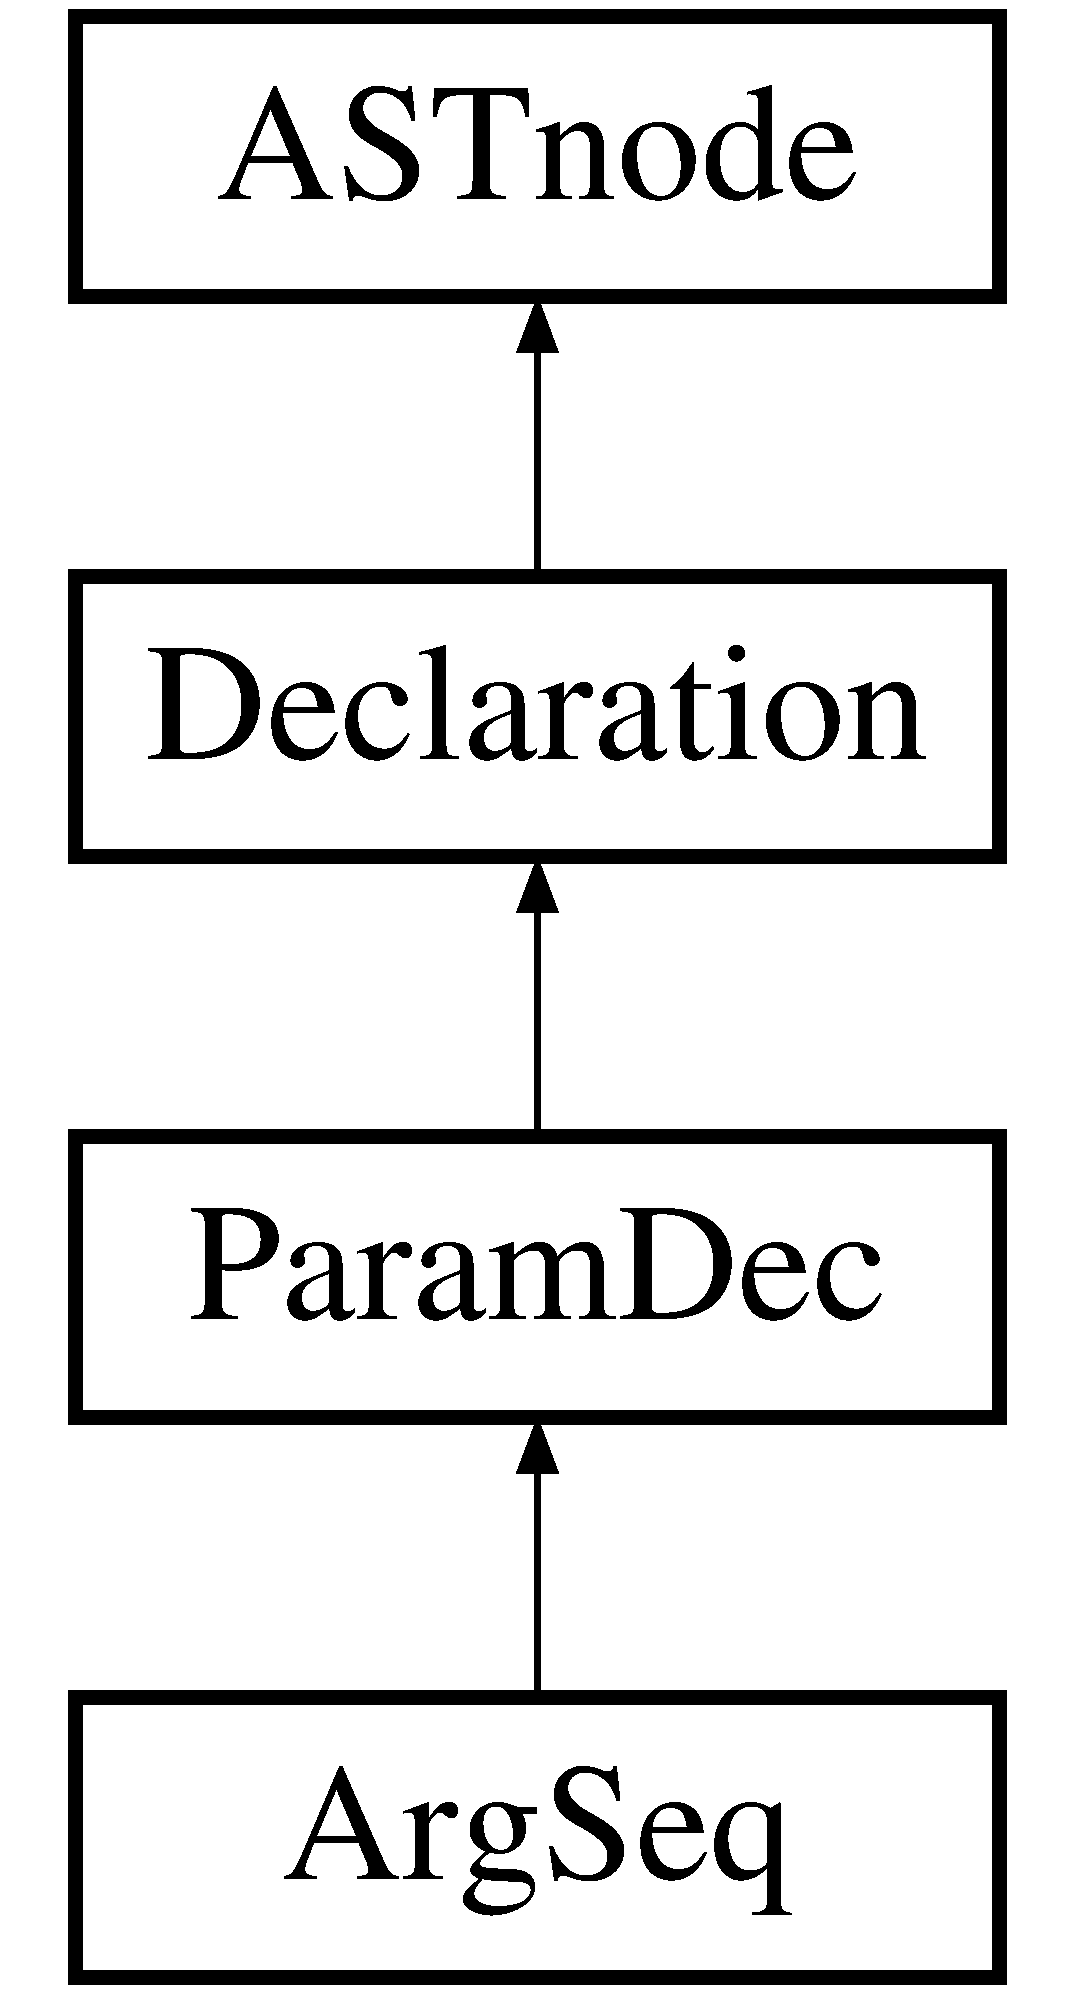
\includegraphics[height=4.000000cm]{class_arg_seq}
\end{center}
\end{figure}
\subsection*{Public Member Functions}
\begin{DoxyCompactItemize}
\item 
\mbox{\Hypertarget{class_arg_seq_af3b662b2cd160ce75f31e1eca76d26da}\label{class_arg_seq_af3b662b2cd160ce75f31e1eca76d26da}} 
int {\bfseries get\+Count} () const
\item 
\mbox{\Hypertarget{class_arg_seq_a3e67a509d46faf71ff827ed1b866ce85}\label{class_arg_seq_a3e67a509d46faf71ff827ed1b866ce85}} 
const \hyperlink{class_expression}{Expression} $\ast$ {\bfseries get\+Declaration} (unsigned int i) const
\item 
\mbox{\Hypertarget{class_arg_seq_a545dc1da22718b659fae03bd69c7dbe8}\label{class_arg_seq_a545dc1da22718b659fae03bd69c7dbe8}} 
void {\bfseries add\+Declaration} (const \hyperlink{class_expression}{Expression} $\ast$state)
\item 
\mbox{\Hypertarget{class_arg_seq_a379b539bc6e8ca25a82308418a135318}\label{class_arg_seq_a379b539bc6e8ca25a82308418a135318}} 
void {\bfseries print} () const override
\item 
\mbox{\Hypertarget{class_arg_seq_aa6124b849889c371a03436601208d03d}\label{class_arg_seq_aa6124b849889c371a03436601208d03d}} 
void {\bfseries compile} (\hyperlink{class_context}{Context} \&ctxt, unsigned int dest\+Loc) const override
\end{DoxyCompactItemize}
\subsection*{Additional Inherited Members}


The documentation for this class was generated from the following files\+:\begin{DoxyCompactItemize}
\item 
ast.\+hpp\item 
ast.\+cpp\end{DoxyCompactItemize}

\hypertarget{class_assignment_statement}{}\section{Assignment\+Statement Class Reference}
\label{class_assignment_statement}\index{Assignment\+Statement@{Assignment\+Statement}}
Inheritance diagram for Assignment\+Statement\+:\begin{figure}[H]
\begin{center}
\leavevmode
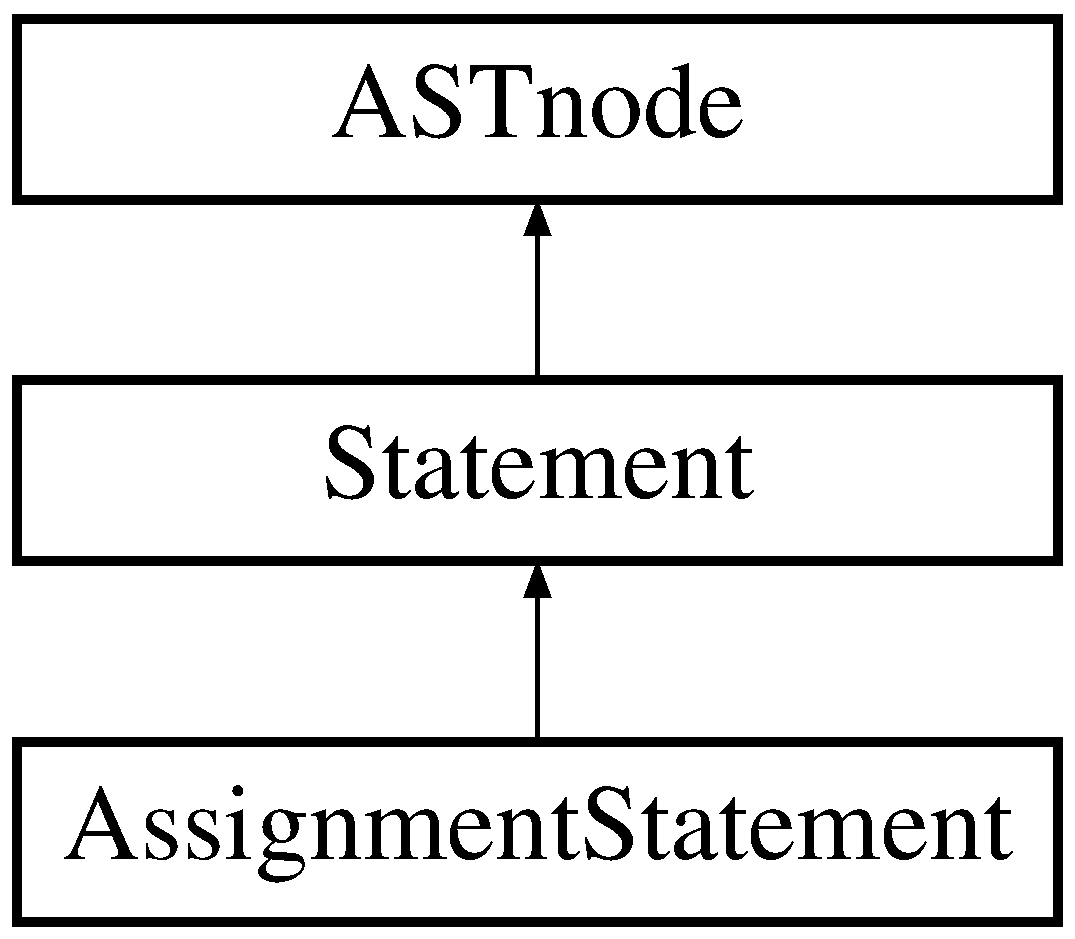
\includegraphics[height=3.000000cm]{class_assignment_statement}
\end{center}
\end{figure}
\subsection*{Public Member Functions}
\begin{DoxyCompactItemize}
\item 
\mbox{\Hypertarget{class_assignment_statement_ab4a99d38ed28b1d6be8274f3118ddce4}\label{class_assignment_statement_ab4a99d38ed28b1d6be8274f3118ddce4}} 
{\bfseries Assignment\+Statement} (const std\+::string $\ast$id\+\_\+in, const \hyperlink{class_expression}{Expression} $\ast$rhs\+\_\+in)
\item 
\mbox{\Hypertarget{class_assignment_statement_a8b312bb1c2b36f359a80b066c9e81c5a}\label{class_assignment_statement_a8b312bb1c2b36f359a80b066c9e81c5a}} 
void {\bfseries print} () const override
\item 
\mbox{\Hypertarget{class_assignment_statement_a8b297acc220822c0d490b67506645915}\label{class_assignment_statement_a8b297acc220822c0d490b67506645915}} 
void {\bfseries compile} (\hyperlink{class_context}{Context} \&ctxt, unsigned int dest\+Loc) const override
\end{DoxyCompactItemize}
\subsection*{Public Attributes}
\begin{DoxyCompactItemize}
\item 
\mbox{\Hypertarget{class_assignment_statement_a78959d944a107ec14ea49639bd3cd473}\label{class_assignment_statement_a78959d944a107ec14ea49639bd3cd473}} 
const std\+::string $\ast$ {\bfseries id}
\item 
\mbox{\Hypertarget{class_assignment_statement_abc3f2374685ba365c72440b8c1c167bc}\label{class_assignment_statement_abc3f2374685ba365c72440b8c1c167bc}} 
const \hyperlink{class_expression}{Expression} $\ast$ {\bfseries rhs}
\end{DoxyCompactItemize}


The documentation for this class was generated from the following files\+:\begin{DoxyCompactItemize}
\item 
ast.\+hpp\item 
ast.\+cpp\end{DoxyCompactItemize}

\hypertarget{class_a_s_tnode}{}\section{A\+S\+Tnode Class Reference}
\label{class_a_s_tnode}\index{A\+S\+Tnode@{A\+S\+Tnode}}
Inheritance diagram for A\+S\+Tnode\+:\begin{figure}[H]
\begin{center}
\leavevmode
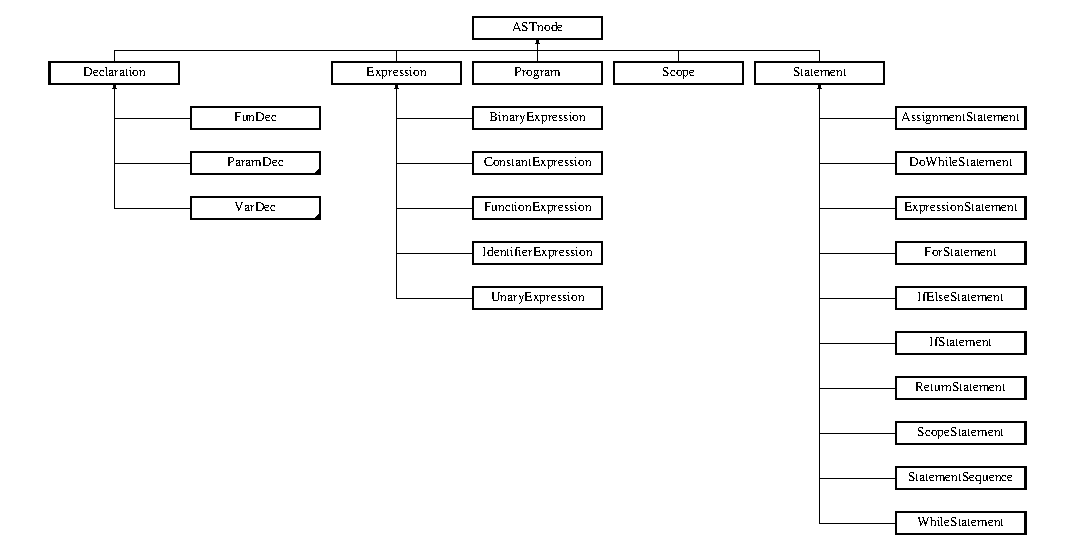
\includegraphics[height=6.956522cm]{class_a_s_tnode}
\end{center}
\end{figure}
\subsection*{Public Member Functions}
\begin{DoxyCompactItemize}
\item 
\mbox{\Hypertarget{class_a_s_tnode_a30c3d4f96b7675f9639d5540eb53470d}\label{class_a_s_tnode_a30c3d4f96b7675f9639d5540eb53470d}} 
virtual void {\bfseries print} () const =0
\item 
\mbox{\Hypertarget{class_a_s_tnode_a45d25ab7b40875c6aedecb9ed41d7d80}\label{class_a_s_tnode_a45d25ab7b40875c6aedecb9ed41d7d80}} 
virtual void {\bfseries compile} (\hyperlink{class_context}{Context} \&ctxt, unsigned int dest\+Loc) const =0
\end{DoxyCompactItemize}


The documentation for this class was generated from the following file\+:\begin{DoxyCompactItemize}
\item 
ast.\+hpp\end{DoxyCompactItemize}

\hypertarget{class_binary_expression}{}\section{Binary\+Expression Class Reference}
\label{class_binary_expression}\index{Binary\+Expression@{Binary\+Expression}}
Inheritance diagram for Binary\+Expression\+:\begin{figure}[H]
\begin{center}
\leavevmode
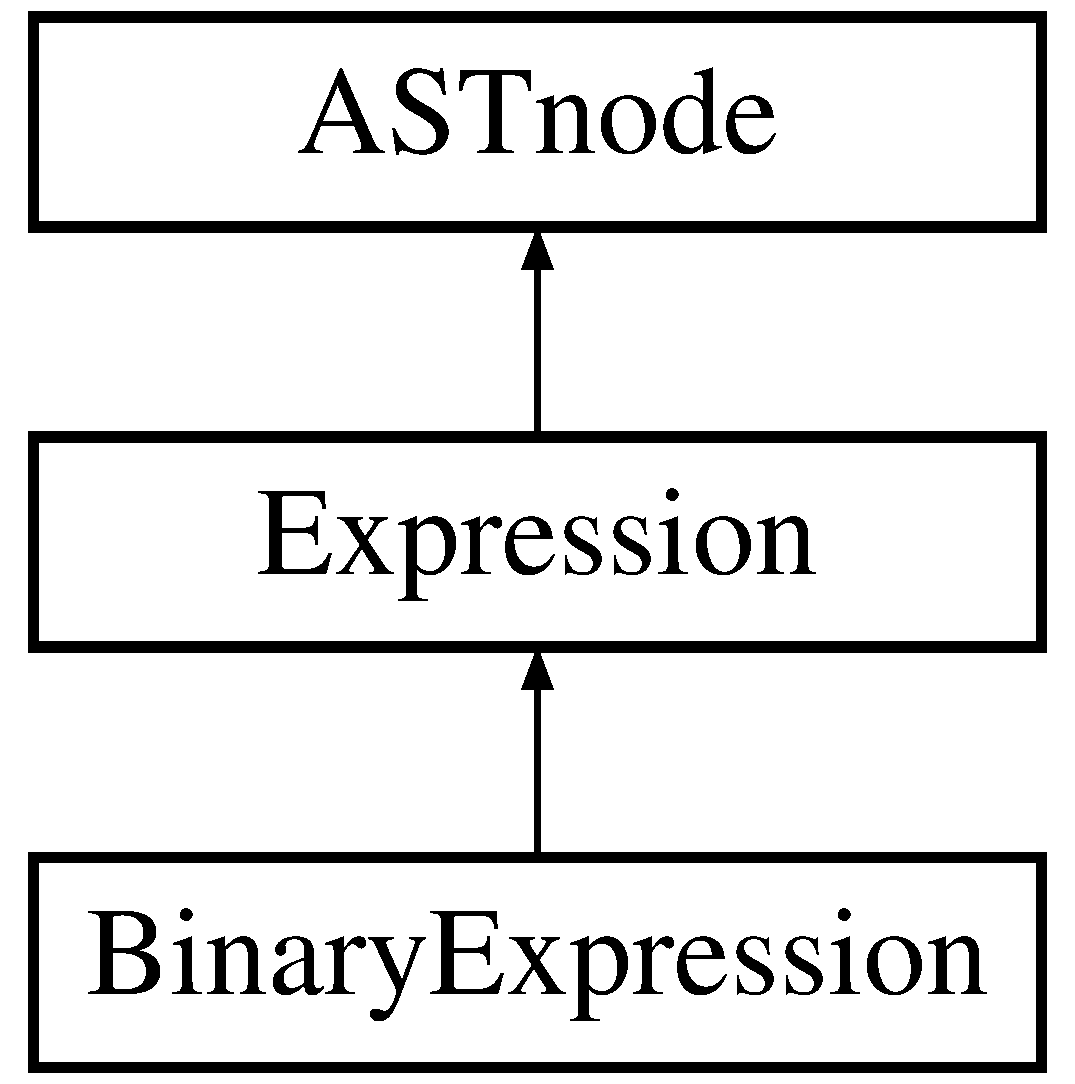
\includegraphics[height=3.000000cm]{class_binary_expression}
\end{center}
\end{figure}
\subsection*{Public Member Functions}
\begin{DoxyCompactItemize}
\item 
\mbox{\Hypertarget{class_binary_expression_a778ec407f2742ef33c7fe443dd8cb9bb}\label{class_binary_expression_a778ec407f2742ef33c7fe443dd8cb9bb}} 
{\bfseries Binary\+Expression} (const \hyperlink{class_expression}{Expression} $\ast$left\+\_\+in, const std\+::string $\ast$op\+\_\+in, const \hyperlink{class_expression}{Expression} $\ast$right\+\_\+in)
\item 
\mbox{\Hypertarget{class_binary_expression_a3083960e3d1f7fe0015f906f20d256e9}\label{class_binary_expression_a3083960e3d1f7fe0015f906f20d256e9}} 
void {\bfseries print} () const override
\item 
\mbox{\Hypertarget{class_binary_expression_a1eaca730f7a3fa6ff8153b23f72eb961}\label{class_binary_expression_a1eaca730f7a3fa6ff8153b23f72eb961}} 
void {\bfseries compile} (\hyperlink{class_context}{Context} \&ctxt, unsigned int dest\+Loc) const override
\end{DoxyCompactItemize}
\subsection*{Public Attributes}
\begin{DoxyCompactItemize}
\item 
\mbox{\Hypertarget{class_binary_expression_a9a5f3daa86c05eace97b8ab081a29544}\label{class_binary_expression_a9a5f3daa86c05eace97b8ab081a29544}} 
const \hyperlink{class_expression}{Expression} $\ast$ {\bfseries left}
\item 
\mbox{\Hypertarget{class_binary_expression_a1124bcd93d45cc8a2639cb1b662ad027}\label{class_binary_expression_a1124bcd93d45cc8a2639cb1b662ad027}} 
const \hyperlink{class_expression}{Expression} $\ast$ {\bfseries right}
\item 
\mbox{\Hypertarget{class_binary_expression_a085e8e782d1370dc7c0a1ae4625654b9}\label{class_binary_expression_a085e8e782d1370dc7c0a1ae4625654b9}} 
const std\+::string $\ast$ {\bfseries op}
\end{DoxyCompactItemize}


The documentation for this class was generated from the following files\+:\begin{DoxyCompactItemize}
\item 
ast.\+hpp\item 
ast.\+cpp\end{DoxyCompactItemize}

\hypertarget{class_constant_expression}{}\section{Constant\+Expression Class Reference}
\label{class_constant_expression}\index{Constant\+Expression@{Constant\+Expression}}
Inheritance diagram for Constant\+Expression\+:\begin{figure}[H]
\begin{center}
\leavevmode
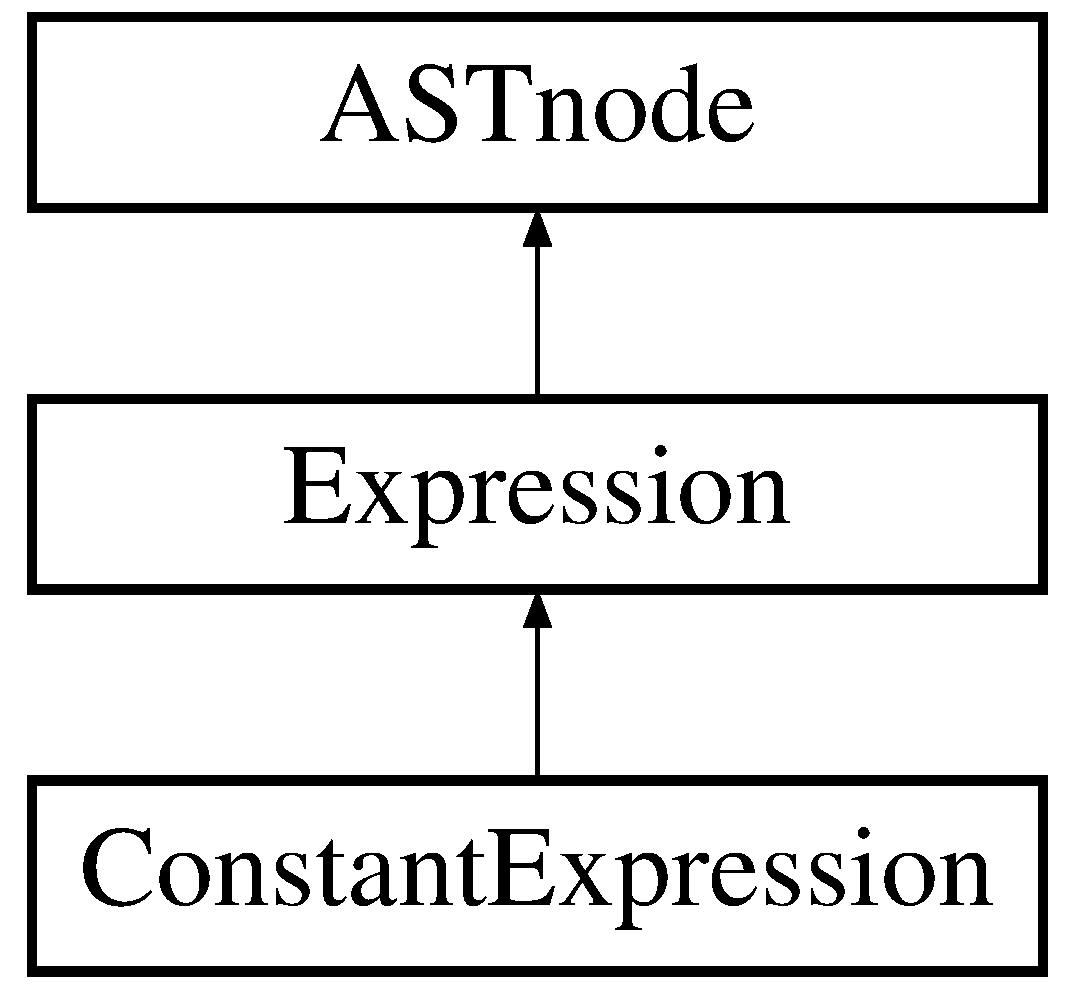
\includegraphics[height=3.000000cm]{class_constant_expression}
\end{center}
\end{figure}
\subsection*{Public Member Functions}
\begin{DoxyCompactItemize}
\item 
\mbox{\Hypertarget{class_constant_expression_a5a620ed4b51118e987acc7ef17b0ed28}\label{class_constant_expression_a5a620ed4b51118e987acc7ef17b0ed28}} 
{\bfseries Constant\+Expression} (const std\+::string $\ast$value\+\_\+in)
\item 
\mbox{\Hypertarget{class_constant_expression_a4039174ef6417f3a74ee6716062221d5}\label{class_constant_expression_a4039174ef6417f3a74ee6716062221d5}} 
void {\bfseries print} () const override
\item 
\mbox{\Hypertarget{class_constant_expression_a833d4384e2e62bf71e8ab95ce68f1c0a}\label{class_constant_expression_a833d4384e2e62bf71e8ab95ce68f1c0a}} 
void {\bfseries compile} (\hyperlink{class_context}{Context} \&ctxt, unsigned int dest\+Loc) const override
\end{DoxyCompactItemize}
\subsection*{Public Attributes}
\begin{DoxyCompactItemize}
\item 
\mbox{\Hypertarget{class_constant_expression_a61f28a690adce4f13a819cb76b77d1f8}\label{class_constant_expression_a61f28a690adce4f13a819cb76b77d1f8}} 
const std\+::string $\ast$ {\bfseries value}
\end{DoxyCompactItemize}


The documentation for this class was generated from the following files\+:\begin{DoxyCompactItemize}
\item 
ast.\+hpp\item 
ast.\+cpp\end{DoxyCompactItemize}

\hypertarget{class_context}{}\section{Context Class Reference}
\label{class_context}\index{Context@{Context}}
\subsection*{Public Member Functions}
\begin{DoxyCompactItemize}
\item 
\mbox{\Hypertarget{class_context_a4fb0726e937fa0ddf829c408f2941ca2}\label{class_context_a4fb0726e937fa0ddf829c408f2941ca2}} 
{\bfseries Context} (\hyperlink{class_context}{Context} $\ast$c)
\item 
\mbox{\Hypertarget{class_context_ad326b2096ae2369d8188eb176d988b70}\label{class_context_ad326b2096ae2369d8188eb176d988b70}} 
std\+::vector$<$ unsigned int $>$ {\bfseries free\+Saved\+Registers} ()
\item 
\mbox{\Hypertarget{class_context_a2a30d44799ac4a9339aa6927b3d56670}\label{class_context_a2a30d44799ac4a9339aa6927b3d56670}} 
std\+::vector$<$ unsigned int $>$ {\bfseries free\+Tmp\+Registers} ()
\item 
\mbox{\Hypertarget{class_context_a13d9bba210a7318e7802d6264ca60eb8}\label{class_context_a13d9bba210a7318e7802d6264ca60eb8}} 
void {\bfseries set\+Used} (unsigned int i)
\item 
\mbox{\Hypertarget{class_context_a1adf3153b961a2eaebf4e8b2e3cbd8bf}\label{class_context_a1adf3153b961a2eaebf4e8b2e3cbd8bf}} 
void {\bfseries set\+Unused} (unsigned int i)
\item 
\mbox{\Hypertarget{class_context_a8dbea6df459519700ec75964690475eb}\label{class_context_a8dbea6df459519700ec75964690475eb}} 
void {\bfseries add\+Global} (const std\+::string $\ast$name)
\item 
\mbox{\Hypertarget{class_context_a2cd8e7b3ee3343f4a0df1f7e0594af0e}\label{class_context_a2cd8e7b3ee3343f4a0df1f7e0594af0e}} 
void {\bfseries delete\+Global} (const std\+::string $\ast$name)
\item 
\mbox{\Hypertarget{class_context_afee1a24074cc55823b8cf516b0c006de}\label{class_context_afee1a24074cc55823b8cf516b0c006de}} 
unsigned int {\bfseries find\+Global} (const std\+::string $\ast$name)
\item 
\mbox{\Hypertarget{class_context_a4392e063038524f16ded5a4727da86ac}\label{class_context_a4392e063038524f16ded5a4727da86ac}} 
bool {\bfseries is\+Global} (const std\+::string $\ast$name)
\item 
\mbox{\Hypertarget{class_context_add5876bef48e55fb6678b1fa66847c02}\label{class_context_add5876bef48e55fb6678b1fa66847c02}} 
void {\bfseries add\+Variable} (const std\+::string $\ast$name)
\item 
\mbox{\Hypertarget{class_context_a1807ed5838267e41a8fd6a2f9746eb5d}\label{class_context_a1807ed5838267e41a8fd6a2f9746eb5d}} 
void {\bfseries delete\+Variable} (const std\+::string $\ast$name)
\item 
\mbox{\Hypertarget{class_context_af0ca1f256d8e85df2776d98641645f6d}\label{class_context_af0ca1f256d8e85df2776d98641645f6d}} 
unsigned int {\bfseries find\+Variable} (const std\+::string $\ast$name)
\item 
\mbox{\Hypertarget{class_context_a3be2ed1410be651593ab477b452b6a74}\label{class_context_a3be2ed1410be651593ab477b452b6a74}} 
bool {\bfseries is\+Variable} (const std\+::string $\ast$name)
\item 
\mbox{\Hypertarget{class_context_a01f91258841aeecffd6d89b243f75dc2}\label{class_context_a01f91258841aeecffd6d89b243f75dc2}} 
void {\bfseries add\+Dynamic} (const std\+::string $\ast$name)
\item 
\mbox{\Hypertarget{class_context_a9bb1b3c01ebbf9f5324f1b52f9c000c6}\label{class_context_a9bb1b3c01ebbf9f5324f1b52f9c000c6}} 
void {\bfseries delete\+Dynamic} (const std\+::string $\ast$name)
\item 
\mbox{\Hypertarget{class_context_abbdfcbf82bca5d5d4bb893323be65f39}\label{class_context_abbdfcbf82bca5d5d4bb893323be65f39}} 
unsigned int {\bfseries find\+Dynamic} (const std\+::string $\ast$name)
\item 
\mbox{\Hypertarget{class_context_ae7b29425bad6cdd9c653ab4d42835393}\label{class_context_ae7b29425bad6cdd9c653ab4d42835393}} 
bool {\bfseries is\+Dynamic} (const std\+::string $\ast$name)
\item 
\mbox{\Hypertarget{class_context_a8dcc97f8f696b8f42bb554658decc369}\label{class_context_a8dcc97f8f696b8f42bb554658decc369}} 
bool {\bfseries is\+On\+Stack} (const std\+::string $\ast$name)
\item 
\mbox{\Hypertarget{class_context_a06f900b507c9013b789c945060bdb684}\label{class_context_a06f900b507c9013b789c945060bdb684}} 
std\+::string {\bfseries find\+On\+Stack} (const std\+::string $\ast$name)
\end{DoxyCompactItemize}
\subsection*{Public Attributes}
\begin{DoxyCompactItemize}
\item 
\mbox{\Hypertarget{class_context_a4154d80f029cc2e348126ca70dd43e94}\label{class_context_a4154d80f029cc2e348126ca70dd43e94}} 
bool {\bfseries regs} \mbox{[}32\mbox{]}
\item 
\mbox{\Hypertarget{class_context_ac383af2b2294500f1cc0370946df81a6}\label{class_context_ac383af2b2294500f1cc0370946df81a6}} 
unsigned int {\bfseries SP}
\item 
\mbox{\Hypertarget{class_context_a9f5e2ccd0d0d14543080829ebf2d4b5b}\label{class_context_a9f5e2ccd0d0d14543080829ebf2d4b5b}} 
unsigned int {\bfseries fsize\+\_\+org}
\item 
\mbox{\Hypertarget{class_context_a3572ac8a19d4afe52f93236158b3ca6b}\label{class_context_a3572ac8a19d4afe52f93236158b3ca6b}} 
unsigned int {\bfseries fsize}
\item 
\mbox{\Hypertarget{class_context_aac2957f7942a067a4d61db0a9d5fa52b}\label{class_context_aac2957f7942a067a4d61db0a9d5fa52b}} 
int {\bfseries param\+No}
\item 
\mbox{\Hypertarget{class_context_a21e93552ced87fbc90e95fb1adefb4d1}\label{class_context_a21e93552ced87fbc90e95fb1adefb4d1}} 
int {\bfseries var\+No}
\item 
\mbox{\Hypertarget{class_context_a1eca674dabc9aacc22cb0b570fcebd46}\label{class_context_a1eca674dabc9aacc22cb0b570fcebd46}} 
int {\bfseries globl\+Var}
\item 
\mbox{\Hypertarget{class_context_a457cedbb97192ceee110548e3b8c0348}\label{class_context_a457cedbb97192ceee110548e3b8c0348}} 
int {\bfseries args\+No}
\item 
\mbox{\Hypertarget{class_context_a789582cf84432865fc58b566c93f79bb}\label{class_context_a789582cf84432865fc58b566c93f79bb}} 
int {\bfseries saved\+No}
\item 
\mbox{\Hypertarget{class_context_af2d41b56e6c75c534ea01e9f9cc7b8de}\label{class_context_af2d41b56e6c75c534ea01e9f9cc7b8de}} 
std\+::unordered\+\_\+map$<$ std\+::string, unsigned int $>$ {\bfseries variable\+Bindings}
\item 
\mbox{\Hypertarget{class_context_a7cd52a34969792c3d414a9d2fb347d79}\label{class_context_a7cd52a34969792c3d414a9d2fb347d79}} 
std\+::unordered\+\_\+map$<$ std\+::string, unsigned int $>$ {\bfseries dynamic\+Bindings}
\item 
\mbox{\Hypertarget{class_context_ab55f4a83656b1385d548507cfaa5e9f4}\label{class_context_ab55f4a83656b1385d548507cfaa5e9f4}} 
std\+::unordered\+\_\+map$<$ std\+::string, unsigned int $>$ {\bfseries global\+Bindings}
\end{DoxyCompactItemize}


The documentation for this class was generated from the following files\+:\begin{DoxyCompactItemize}
\item 
context.\+hpp\item 
context.\+cpp\end{DoxyCompactItemize}

\hypertarget{class_declaration}{}\section{Declaration Class Reference}
\label{class_declaration}\index{Declaration@{Declaration}}
Inheritance diagram for Declaration\+:\begin{figure}[H]
\begin{center}
\leavevmode
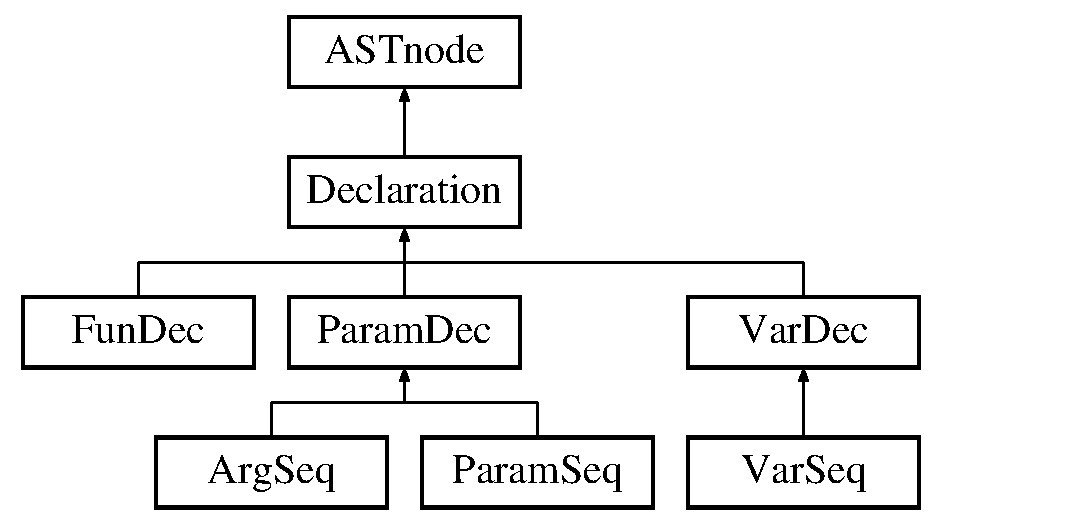
\includegraphics[height=4.000000cm]{class_declaration}
\end{center}
\end{figure}
\subsection*{Public Member Functions}
\begin{DoxyCompactItemize}
\item 
\mbox{\Hypertarget{class_declaration_a40b12f4c11d0111a207ba46be46468e0}\label{class_declaration_a40b12f4c11d0111a207ba46be46468e0}} 
virtual void {\bfseries print} () const =0
\item 
\mbox{\Hypertarget{class_declaration_ab5851fc955e24903f06849c0c1ec74d3}\label{class_declaration_ab5851fc955e24903f06849c0c1ec74d3}} 
virtual void {\bfseries compile} (\hyperlink{class_context}{Context} \&ctxt, unsigned int dest\+Loc) const =0
\end{DoxyCompactItemize}


The documentation for this class was generated from the following file\+:\begin{DoxyCompactItemize}
\item 
ast.\+hpp\end{DoxyCompactItemize}

\hypertarget{class_do_while_statement}{}\section{Do\+While\+Statement Class Reference}
\label{class_do_while_statement}\index{Do\+While\+Statement@{Do\+While\+Statement}}
Inheritance diagram for Do\+While\+Statement\+:\begin{figure}[H]
\begin{center}
\leavevmode
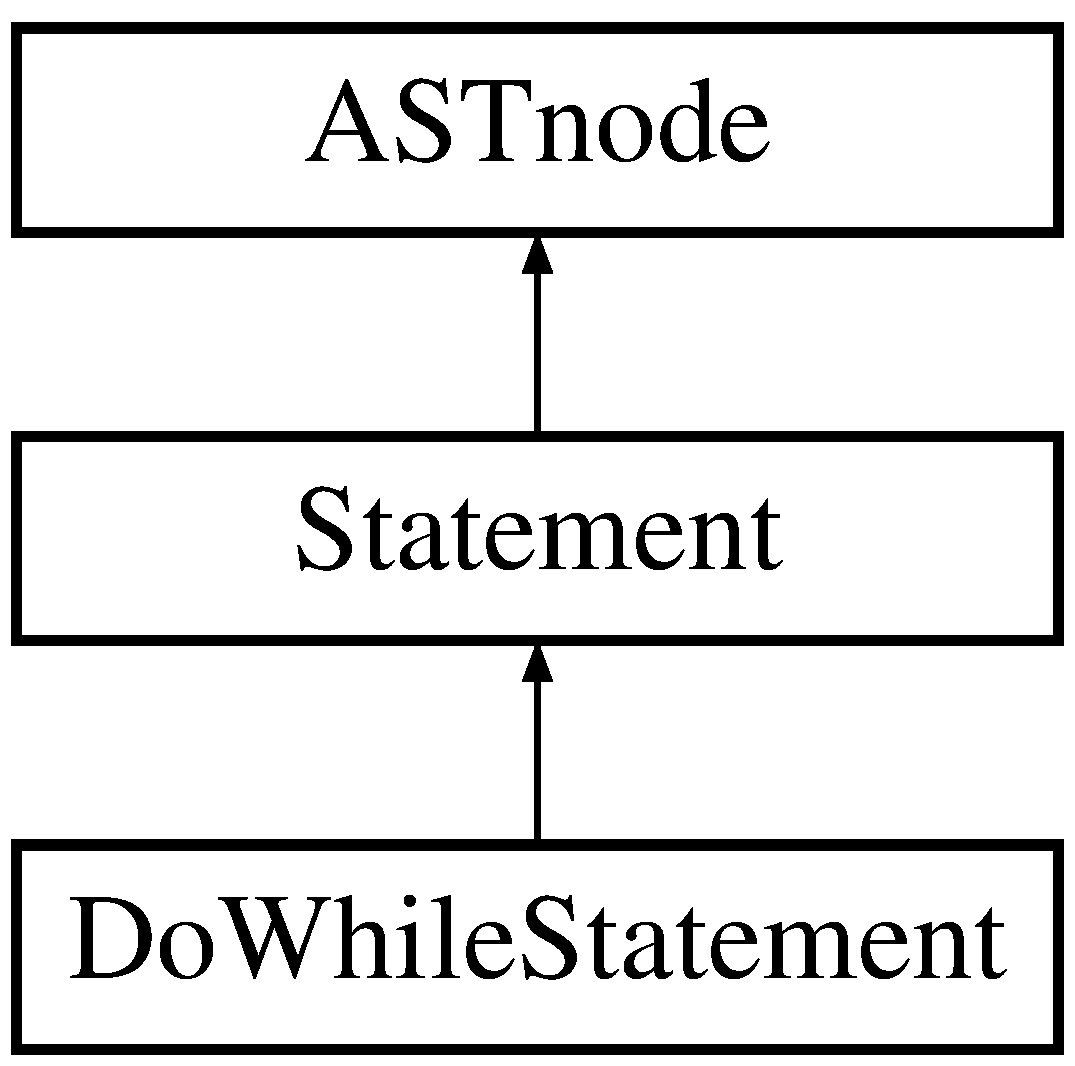
\includegraphics[height=3.000000cm]{class_do_while_statement}
\end{center}
\end{figure}
\subsection*{Public Member Functions}
\begin{DoxyCompactItemize}
\item 
\mbox{\Hypertarget{class_do_while_statement_ab9d1bb6ed026a6fd502cba0fbe02b032}\label{class_do_while_statement_ab9d1bb6ed026a6fd502cba0fbe02b032}} 
{\bfseries Do\+While\+Statement} (\hyperlink{class_scope}{Scope} $\ast$body\+\_\+in, const \hyperlink{class_expression}{Expression} $\ast$cond\+\_\+in)
\item 
\mbox{\Hypertarget{class_do_while_statement_ab870167480b6bec4854dbc9fae60f769}\label{class_do_while_statement_ab870167480b6bec4854dbc9fae60f769}} 
void {\bfseries print} () const override
\item 
\mbox{\Hypertarget{class_do_while_statement_a84a05bbf293d37c869afc13798a34043}\label{class_do_while_statement_a84a05bbf293d37c869afc13798a34043}} 
void {\bfseries compile} (\hyperlink{class_context}{Context} \&ctxt, unsigned int dest\+Loc) const override
\end{DoxyCompactItemize}
\subsection*{Public Attributes}
\begin{DoxyCompactItemize}
\item 
\mbox{\Hypertarget{class_do_while_statement_a94d6fe1ebbc26b2ee9bbb1450a9570e7}\label{class_do_while_statement_a94d6fe1ebbc26b2ee9bbb1450a9570e7}} 
\hyperlink{class_scope}{Scope} $\ast$ {\bfseries body}
\item 
\mbox{\Hypertarget{class_do_while_statement_ad16e911c382c07b4323d873103044596}\label{class_do_while_statement_ad16e911c382c07b4323d873103044596}} 
const \hyperlink{class_expression}{Expression} $\ast$ {\bfseries condition}
\end{DoxyCompactItemize}


The documentation for this class was generated from the following files\+:\begin{DoxyCompactItemize}
\item 
ast.\+hpp\item 
ast.\+cpp\end{DoxyCompactItemize}

\hypertarget{class_expression}{}\section{Expression Class Reference}
\label{class_expression}\index{Expression@{Expression}}
Inheritance diagram for Expression\+:\begin{figure}[H]
\begin{center}
\leavevmode
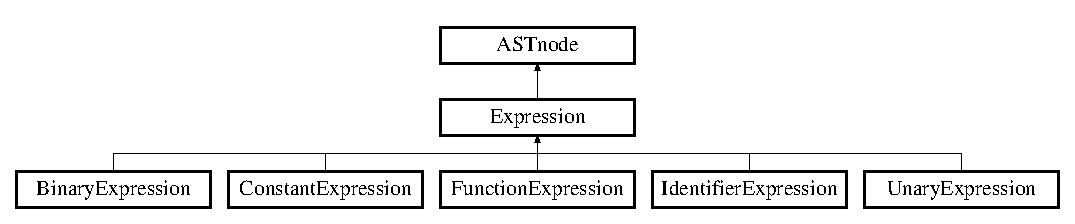
\includegraphics[height=2.564885cm]{class_expression}
\end{center}
\end{figure}
\subsection*{Public Member Functions}
\begin{DoxyCompactItemize}
\item 
\mbox{\Hypertarget{class_expression_ae11e78376212134745e5fa9f0b91dbd1}\label{class_expression_ae11e78376212134745e5fa9f0b91dbd1}} 
virtual void {\bfseries print} () const =0
\item 
\mbox{\Hypertarget{class_expression_af8973027899fe2dcd3fb91cfc52e7eb6}\label{class_expression_af8973027899fe2dcd3fb91cfc52e7eb6}} 
virtual void {\bfseries compile} (\hyperlink{class_context}{Context} \&ctxt, unsigned int dest\+Loc) const =0
\end{DoxyCompactItemize}


The documentation for this class was generated from the following file\+:\begin{DoxyCompactItemize}
\item 
ast.\+hpp\end{DoxyCompactItemize}

\hypertarget{class_expression_statement}{}\section{Expression\+Statement Class Reference}
\label{class_expression_statement}\index{Expression\+Statement@{Expression\+Statement}}
Inheritance diagram for Expression\+Statement\+:\begin{figure}[H]
\begin{center}
\leavevmode
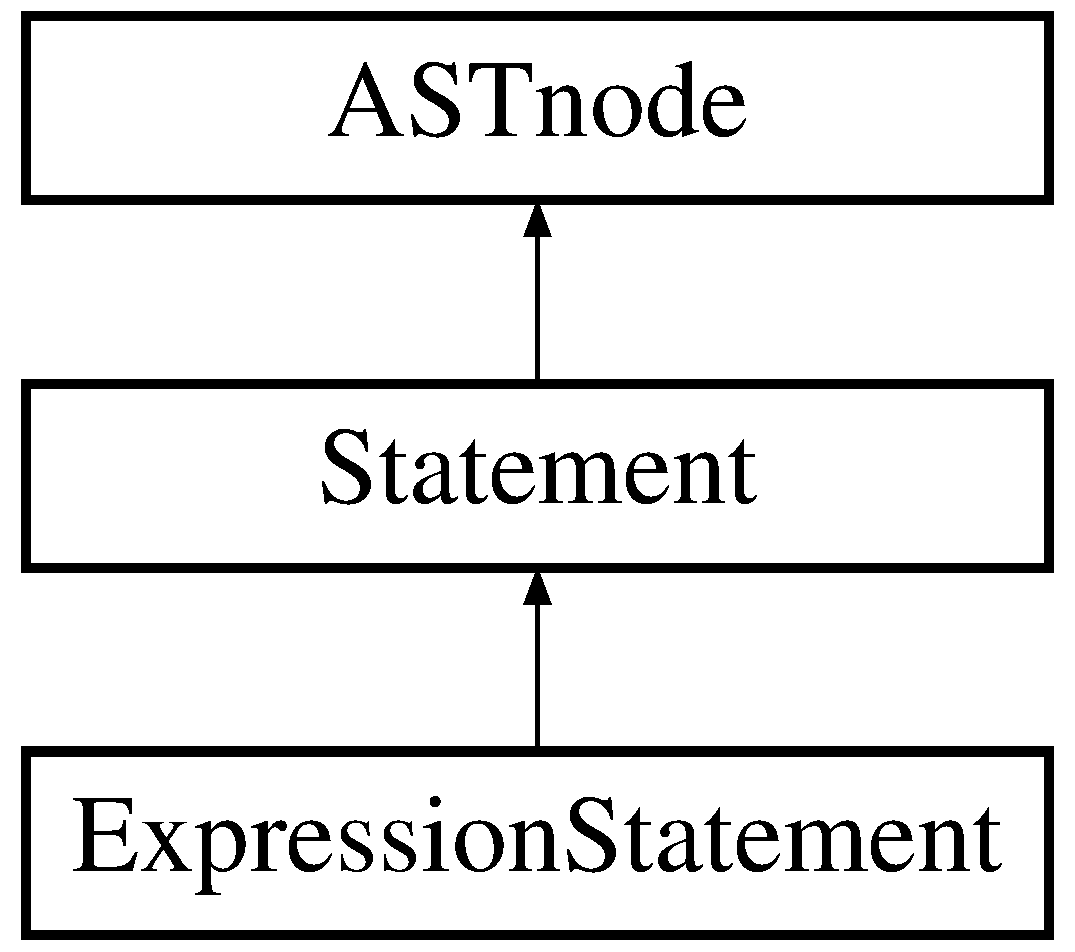
\includegraphics[height=3.000000cm]{class_expression_statement}
\end{center}
\end{figure}
\subsection*{Public Member Functions}
\begin{DoxyCompactItemize}
\item 
\mbox{\Hypertarget{class_expression_statement_a059afaa2d2b18fc3ce504637436f1fa2}\label{class_expression_statement_a059afaa2d2b18fc3ce504637436f1fa2}} 
{\bfseries Expression\+Statement} (const \hyperlink{class_expression}{Expression} $\ast$expr\+\_\+in)
\item 
\mbox{\Hypertarget{class_expression_statement_a1b2b835d8b55c0fe7ed5c36a91ac0e38}\label{class_expression_statement_a1b2b835d8b55c0fe7ed5c36a91ac0e38}} 
void {\bfseries print} () const override
\item 
\mbox{\Hypertarget{class_expression_statement_aefe0183e77528168ce58575d0ddf3bc2}\label{class_expression_statement_aefe0183e77528168ce58575d0ddf3bc2}} 
void {\bfseries compile} (\hyperlink{class_context}{Context} \&ctxt, unsigned int dest\+Loc) const override
\end{DoxyCompactItemize}
\subsection*{Public Attributes}
\begin{DoxyCompactItemize}
\item 
\mbox{\Hypertarget{class_expression_statement_a30a0a5bbd251c79a62708ca201874738}\label{class_expression_statement_a30a0a5bbd251c79a62708ca201874738}} 
const \hyperlink{class_expression}{Expression} $\ast$ {\bfseries expression}
\end{DoxyCompactItemize}


The documentation for this class was generated from the following files\+:\begin{DoxyCompactItemize}
\item 
ast.\+hpp\item 
ast.\+cpp\end{DoxyCompactItemize}

\hypertarget{class_for_statement}{}\section{For\+Statement Class Reference}
\label{class_for_statement}\index{For\+Statement@{For\+Statement}}
Inheritance diagram for For\+Statement\+:\begin{figure}[H]
\begin{center}
\leavevmode
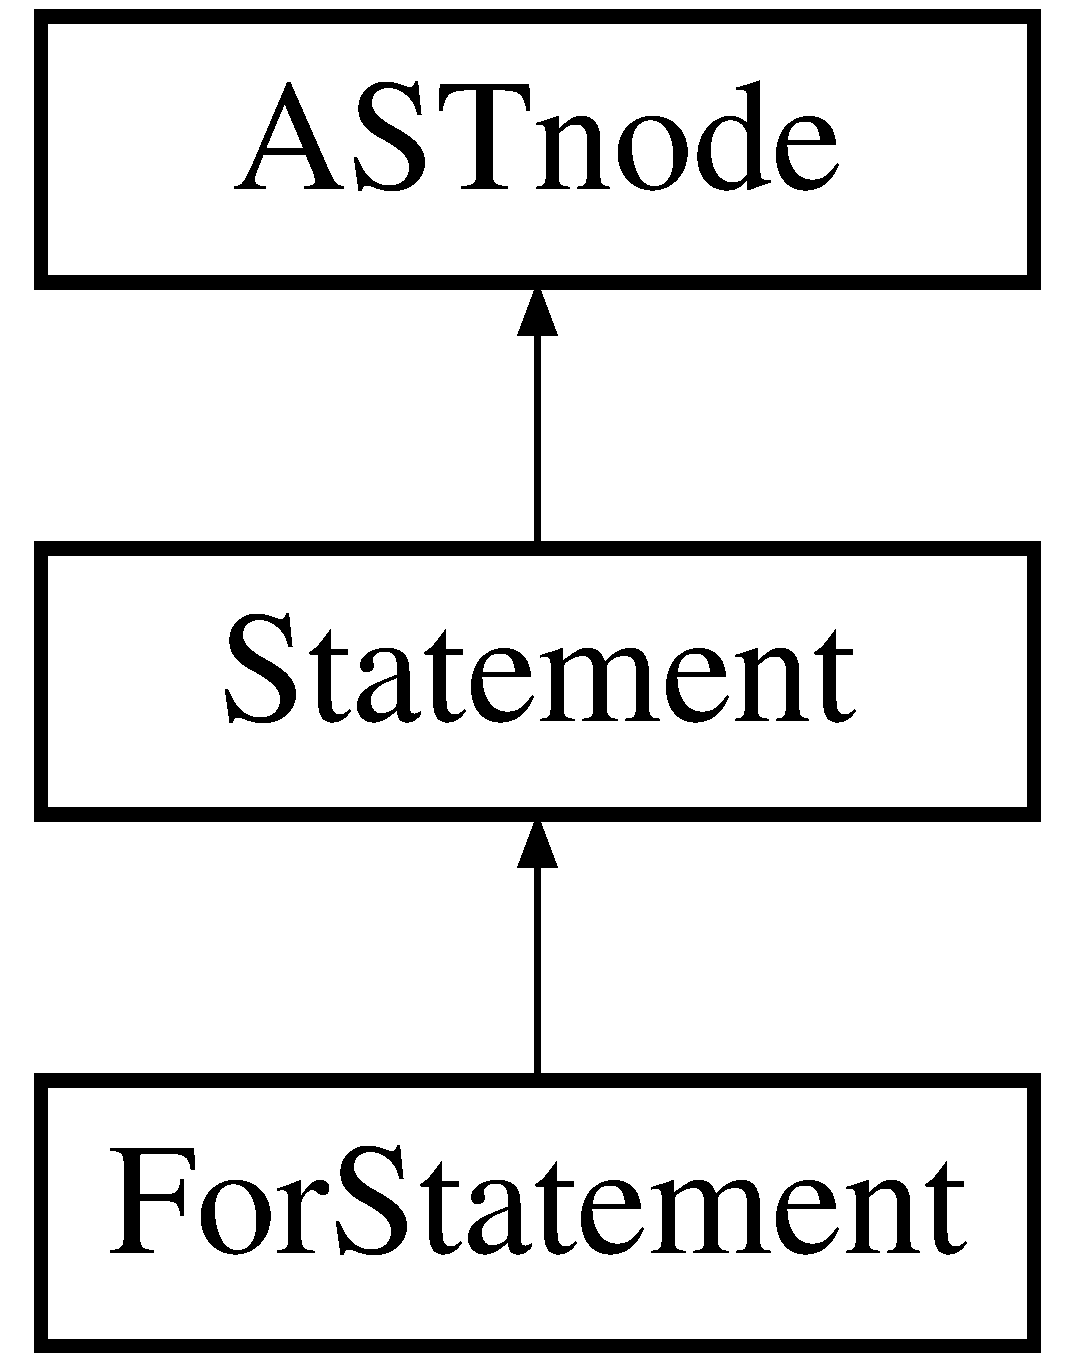
\includegraphics[height=3.000000cm]{class_for_statement}
\end{center}
\end{figure}
\subsection*{Public Member Functions}
\begin{DoxyCompactItemize}
\item 
\mbox{\Hypertarget{class_for_statement_ae97d7b04d1286c2526afea1334ed3b5c}\label{class_for_statement_ae97d7b04d1286c2526afea1334ed3b5c}} 
{\bfseries For\+Statement} (const \hyperlink{class_statement}{Statement} $\ast$init\+\_\+in, const \hyperlink{class_statement}{Statement} $\ast$cond\+\_\+in, const \hyperlink{class_statement}{Statement} $\ast$step\+\_\+in, \hyperlink{class_scope}{Scope} $\ast$body\+\_\+in)
\item 
\mbox{\Hypertarget{class_for_statement_a4cd6e716523339630163e9ed6a40d871}\label{class_for_statement_a4cd6e716523339630163e9ed6a40d871}} 
void {\bfseries print} () const override
\item 
\mbox{\Hypertarget{class_for_statement_affb13212c8806cf22daf04881f488511}\label{class_for_statement_affb13212c8806cf22daf04881f488511}} 
void {\bfseries compile} (\hyperlink{class_context}{Context} \&ctxt, unsigned int dest\+Loc) const override
\end{DoxyCompactItemize}
\subsection*{Public Attributes}
\begin{DoxyCompactItemize}
\item 
\mbox{\Hypertarget{class_for_statement_ac9e5f93a508f56a77e69c4245333f0ae}\label{class_for_statement_ac9e5f93a508f56a77e69c4245333f0ae}} 
const \hyperlink{class_statement}{Statement} $\ast$ {\bfseries init}
\item 
\mbox{\Hypertarget{class_for_statement_ac5ec9bf9fee699436e8e41548e83855c}\label{class_for_statement_ac5ec9bf9fee699436e8e41548e83855c}} 
const \hyperlink{class_statement}{Statement} $\ast$ {\bfseries condition}
\item 
\mbox{\Hypertarget{class_for_statement_abf5f0ce2b90c9420eee55e14ec8edec5}\label{class_for_statement_abf5f0ce2b90c9420eee55e14ec8edec5}} 
const \hyperlink{class_statement}{Statement} $\ast$ {\bfseries step}
\item 
\mbox{\Hypertarget{class_for_statement_a5f9a886aa5ce770c6d5ecb0df1d7b191}\label{class_for_statement_a5f9a886aa5ce770c6d5ecb0df1d7b191}} 
\hyperlink{class_scope}{Scope} $\ast$ {\bfseries body}
\end{DoxyCompactItemize}


The documentation for this class was generated from the following files\+:\begin{DoxyCompactItemize}
\item 
ast.\+hpp\item 
ast.\+cpp\end{DoxyCompactItemize}

\hypertarget{class_function_expression}{}\section{Function\+Expression Class Reference}
\label{class_function_expression}\index{Function\+Expression@{Function\+Expression}}
Inheritance diagram for Function\+Expression\+:\begin{figure}[H]
\begin{center}
\leavevmode
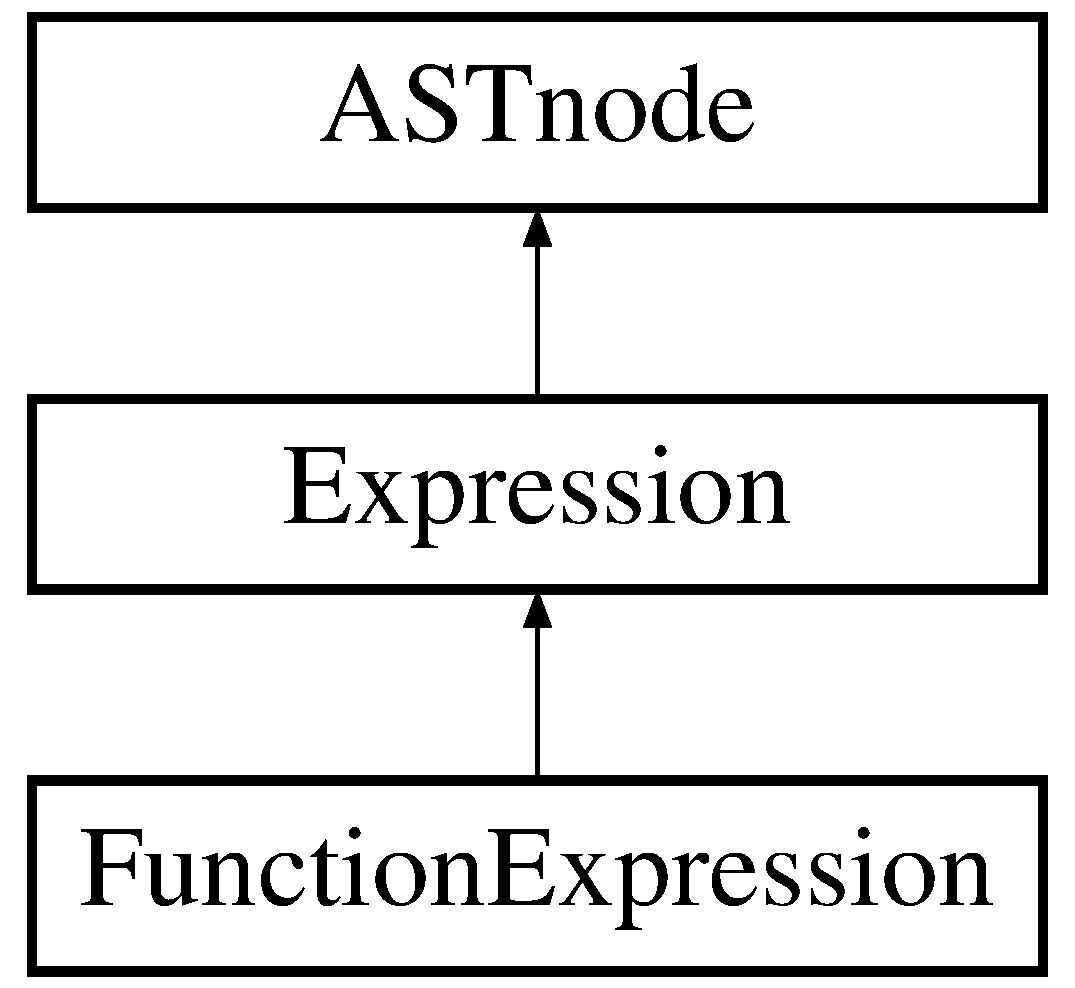
\includegraphics[height=3.000000cm]{class_function_expression}
\end{center}
\end{figure}
\subsection*{Public Member Functions}
\begin{DoxyCompactItemize}
\item 
\mbox{\Hypertarget{class_function_expression_a94946fa67e5e4183faf46eadcb1b2eef}\label{class_function_expression_a94946fa67e5e4183faf46eadcb1b2eef}} 
{\bfseries Function\+Expression} (const std\+::string $\ast$name\+\_\+in, \hyperlink{class_arg_seq}{Arg\+Seq} $\ast$args\+\_\+in)
\item 
\mbox{\Hypertarget{class_function_expression_a5027d5ca974d3aa426cffdb5408266f3}\label{class_function_expression_a5027d5ca974d3aa426cffdb5408266f3}} 
void {\bfseries print} () const override
\item 
\mbox{\Hypertarget{class_function_expression_a83d0abae2f3b3120339aa18a115bdf8a}\label{class_function_expression_a83d0abae2f3b3120339aa18a115bdf8a}} 
void {\bfseries compile} (\hyperlink{class_context}{Context} \&ctxt, unsigned int dest\+Loc) const override
\end{DoxyCompactItemize}
\subsection*{Public Attributes}
\begin{DoxyCompactItemize}
\item 
\mbox{\Hypertarget{class_function_expression_a83d909ec6471c112132860f8410945aa}\label{class_function_expression_a83d909ec6471c112132860f8410945aa}} 
const std\+::string $\ast$ {\bfseries name}
\item 
\mbox{\Hypertarget{class_function_expression_a26950b4622b292d4594dcc1ce9d6e4bc}\label{class_function_expression_a26950b4622b292d4594dcc1ce9d6e4bc}} 
\hyperlink{class_arg_seq}{Arg\+Seq} $\ast$ {\bfseries args}
\end{DoxyCompactItemize}


The documentation for this class was generated from the following files\+:\begin{DoxyCompactItemize}
\item 
ast.\+hpp\item 
ast.\+cpp\end{DoxyCompactItemize}

\hypertarget{class_fun_dec}{}\section{Fun\+Dec Class Reference}
\label{class_fun_dec}\index{Fun\+Dec@{Fun\+Dec}}
Inheritance diagram for Fun\+Dec\+:\begin{figure}[H]
\begin{center}
\leavevmode
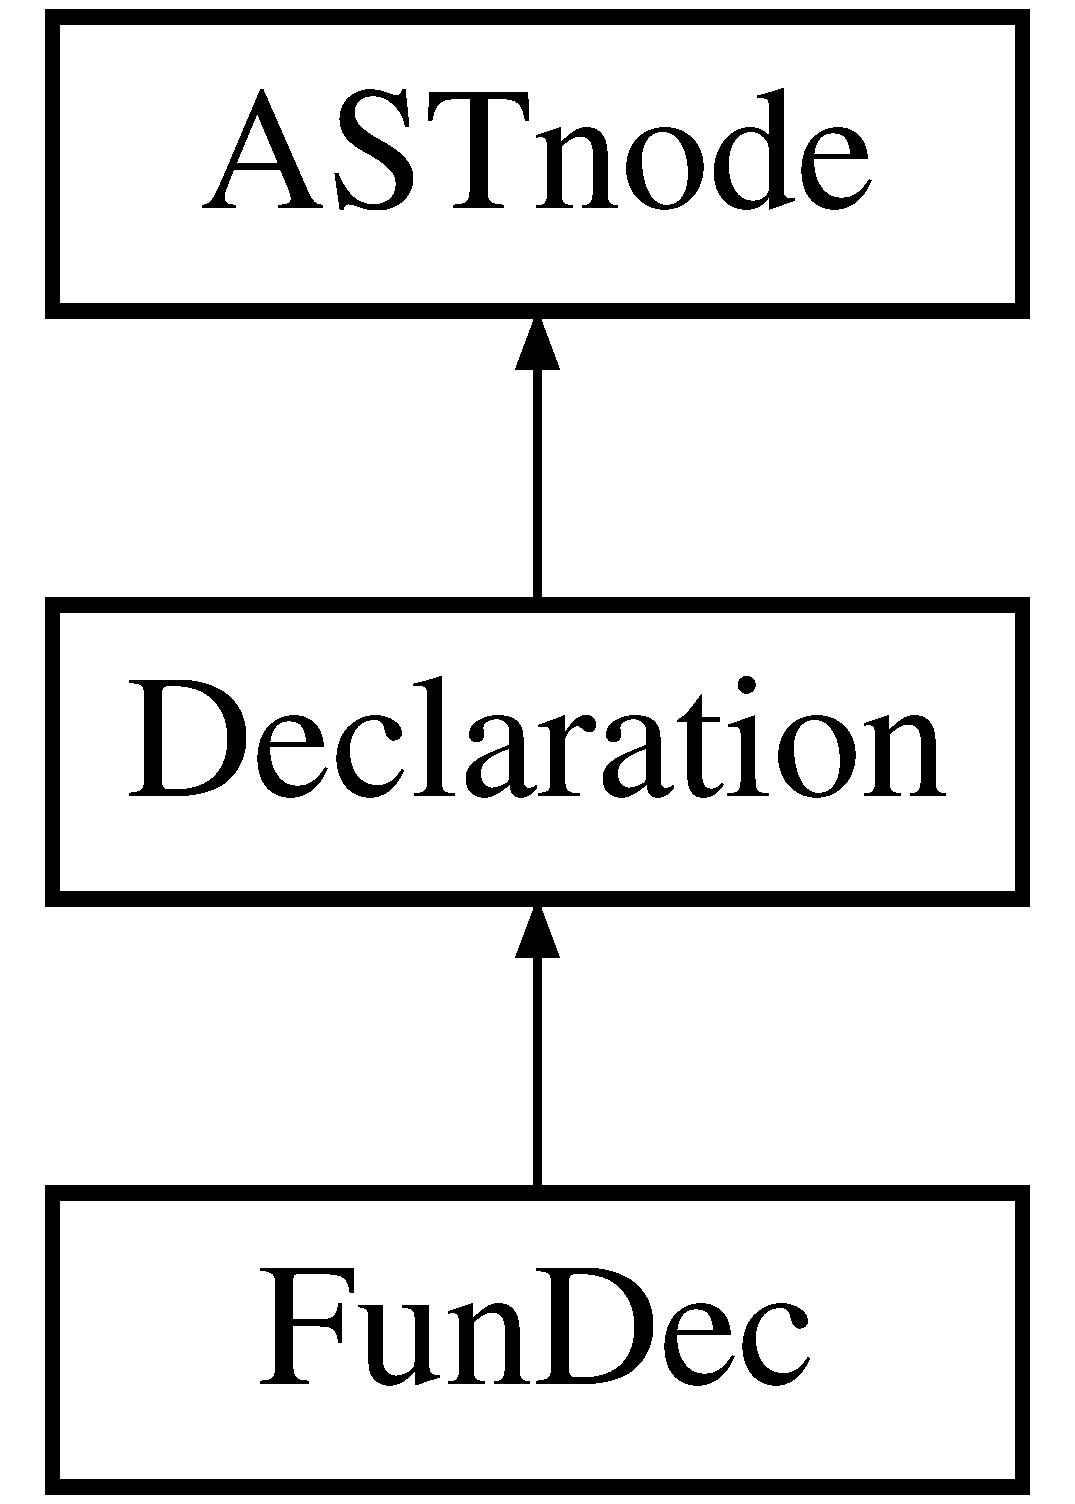
\includegraphics[height=3.000000cm]{class_fun_dec}
\end{center}
\end{figure}
\subsection*{Public Member Functions}
\begin{DoxyCompactItemize}
\item 
\mbox{\Hypertarget{class_fun_dec_abb5640a7ff921a46153d65b085d3f418}\label{class_fun_dec_abb5640a7ff921a46153d65b085d3f418}} 
{\bfseries Fun\+Dec} (const std\+::string $\ast$\+\_\+type, const std\+::string $\ast$\+\_\+id, \hyperlink{class_param_seq}{Param\+Seq} $\ast$param, \hyperlink{class_scope}{Scope} $\ast$body)
\item 
\mbox{\Hypertarget{class_fun_dec_a3173002f9e06597f1bc6946dad5e82ea}\label{class_fun_dec_a3173002f9e06597f1bc6946dad5e82ea}} 
void {\bfseries print} () const override
\item 
\mbox{\Hypertarget{class_fun_dec_ac33111c84de9dbc2e268f0c3de0a3d66}\label{class_fun_dec_ac33111c84de9dbc2e268f0c3de0a3d66}} 
void {\bfseries compile} (\hyperlink{class_context}{Context} \&ctxt, unsigned int dest\+Loc) const override
\end{DoxyCompactItemize}
\subsection*{Public Attributes}
\begin{DoxyCompactItemize}
\item 
\mbox{\Hypertarget{class_fun_dec_aa0b19bf88acf2d9b23ba4ede1e8ede0b}\label{class_fun_dec_aa0b19bf88acf2d9b23ba4ede1e8ede0b}} 
const std\+::string $\ast$ {\bfseries type}
\item 
\mbox{\Hypertarget{class_fun_dec_a0fbbe98cd292b02d6268a448cb05aeea}\label{class_fun_dec_a0fbbe98cd292b02d6268a448cb05aeea}} 
const std\+::string $\ast$ {\bfseries id}
\item 
\mbox{\Hypertarget{class_fun_dec_aa5e931e5491a83372139f0afdf3156cc}\label{class_fun_dec_aa5e931e5491a83372139f0afdf3156cc}} 
\hyperlink{class_param_seq}{Param\+Seq} $\ast$ {\bfseries parameters}
\item 
\mbox{\Hypertarget{class_fun_dec_a4c67d8e464a02b76518327537f5247be}\label{class_fun_dec_a4c67d8e464a02b76518327537f5247be}} 
\hyperlink{class_scope}{Scope} $\ast$ {\bfseries body}
\end{DoxyCompactItemize}


The documentation for this class was generated from the following files\+:\begin{DoxyCompactItemize}
\item 
ast.\+hpp\item 
ast.\+cpp\end{DoxyCompactItemize}

\hypertarget{class_identifier_expression}{}\section{Identifier\+Expression Class Reference}
\label{class_identifier_expression}\index{Identifier\+Expression@{Identifier\+Expression}}
Inheritance diagram for Identifier\+Expression\+:\begin{figure}[H]
\begin{center}
\leavevmode
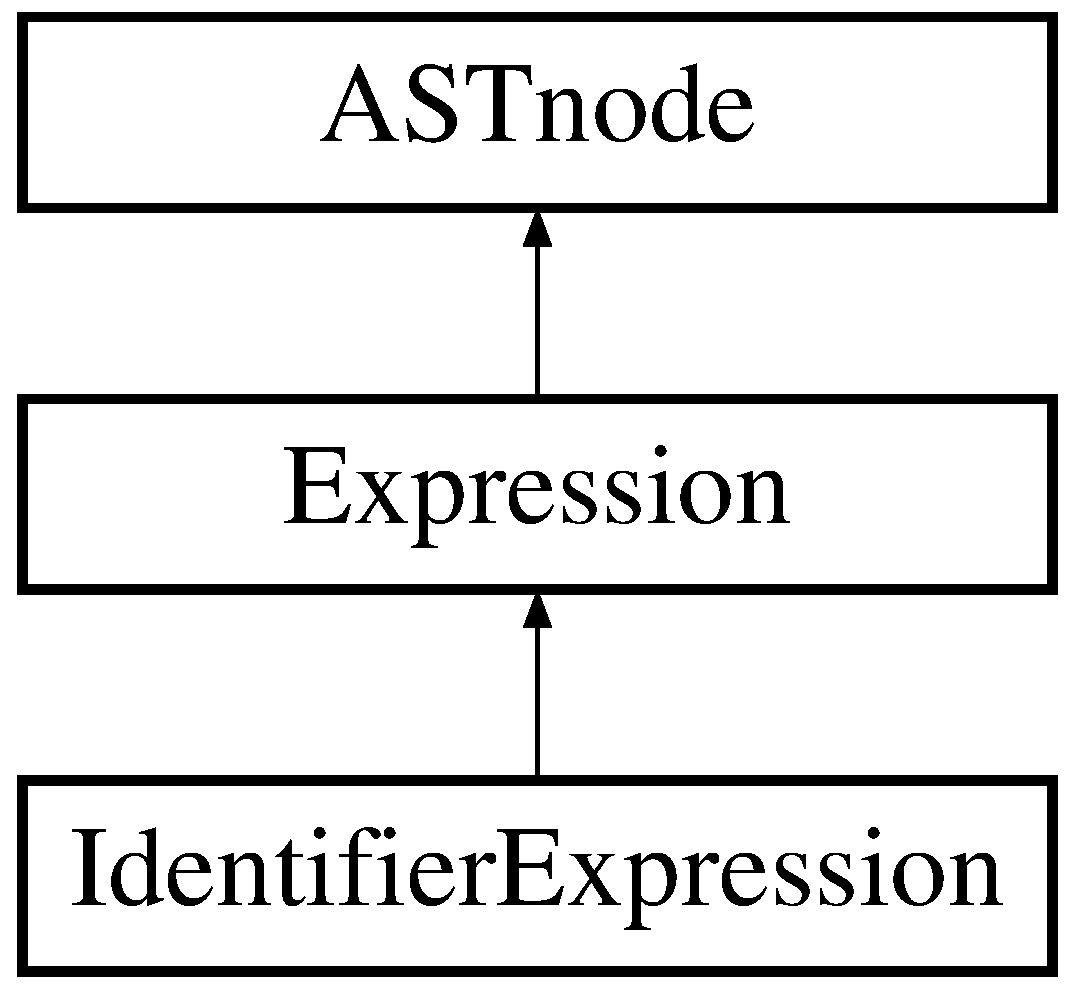
\includegraphics[height=3.000000cm]{class_identifier_expression}
\end{center}
\end{figure}
\subsection*{Public Member Functions}
\begin{DoxyCompactItemize}
\item 
\mbox{\Hypertarget{class_identifier_expression_a471958b271d841936ea341349af2c921}\label{class_identifier_expression_a471958b271d841936ea341349af2c921}} 
{\bfseries Identifier\+Expression} (const std\+::string $\ast$name\+\_\+in)
\item 
\mbox{\Hypertarget{class_identifier_expression_a832327eff23e31cf8378c71c46d4d894}\label{class_identifier_expression_a832327eff23e31cf8378c71c46d4d894}} 
void {\bfseries print} () const override
\item 
\mbox{\Hypertarget{class_identifier_expression_aeb7d933cae1a1e81affc9ac6c887cf10}\label{class_identifier_expression_aeb7d933cae1a1e81affc9ac6c887cf10}} 
void {\bfseries compile} (\hyperlink{class_context}{Context} \&ctxt, unsigned int dest\+Loc) const override
\end{DoxyCompactItemize}
\subsection*{Public Attributes}
\begin{DoxyCompactItemize}
\item 
\mbox{\Hypertarget{class_identifier_expression_a0420bfd651f78cd02094288b72878821}\label{class_identifier_expression_a0420bfd651f78cd02094288b72878821}} 
const std\+::string $\ast$ {\bfseries name}
\end{DoxyCompactItemize}


The documentation for this class was generated from the following files\+:\begin{DoxyCompactItemize}
\item 
ast.\+hpp\item 
ast.\+cpp\end{DoxyCompactItemize}

\hypertarget{class_if_else_statement}{}\section{If\+Else\+Statement Class Reference}
\label{class_if_else_statement}\index{If\+Else\+Statement@{If\+Else\+Statement}}
Inheritance diagram for If\+Else\+Statement\+:\begin{figure}[H]
\begin{center}
\leavevmode
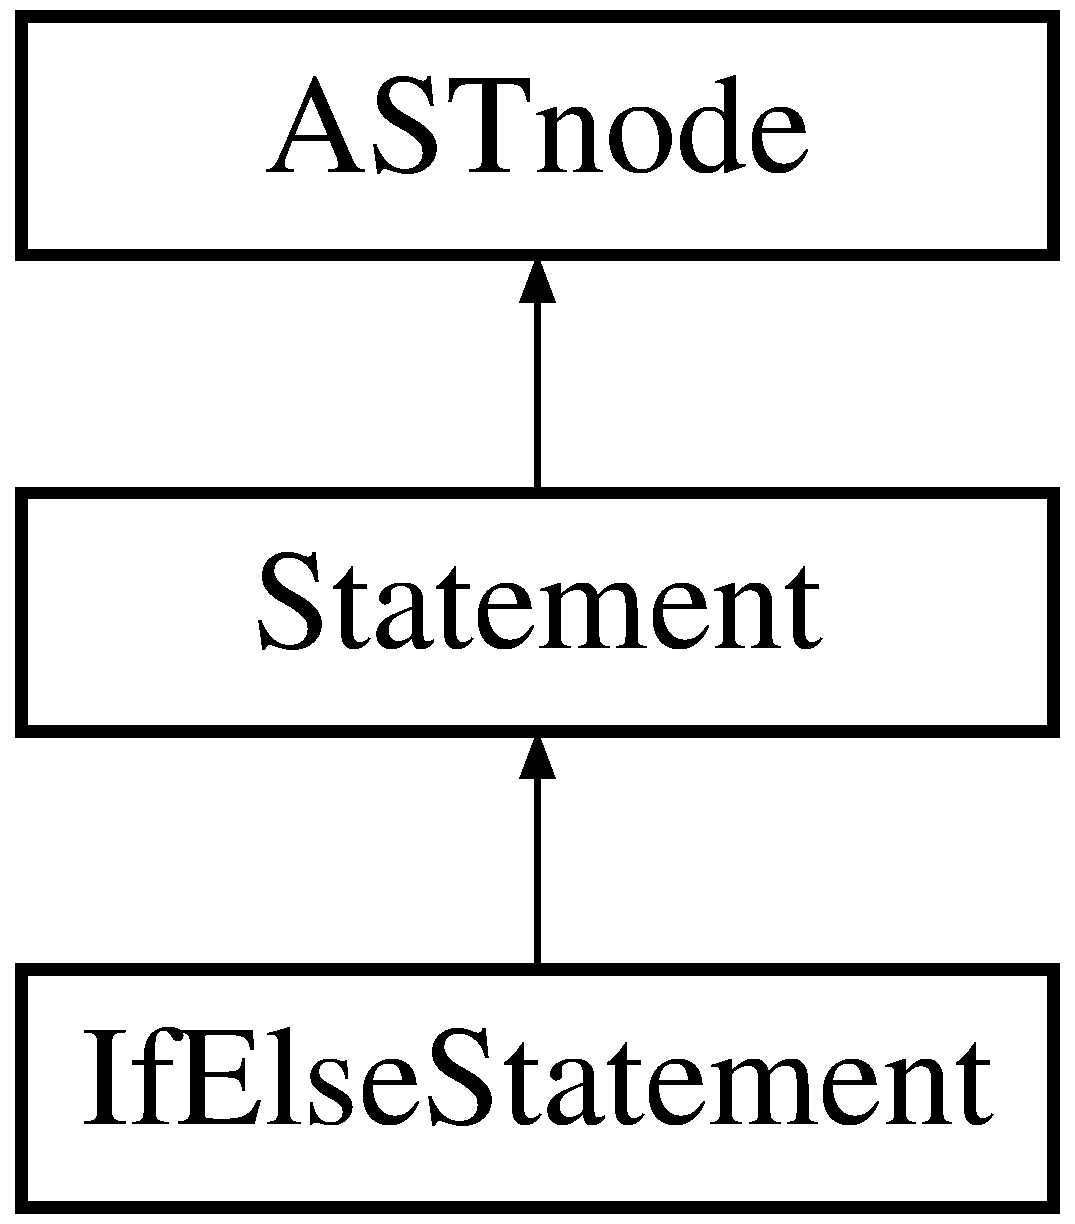
\includegraphics[height=3.000000cm]{class_if_else_statement}
\end{center}
\end{figure}
\subsection*{Public Member Functions}
\begin{DoxyCompactItemize}
\item 
\mbox{\Hypertarget{class_if_else_statement_a1838077ebc90cfc5309fe0e2acad5d16}\label{class_if_else_statement_a1838077ebc90cfc5309fe0e2acad5d16}} 
{\bfseries If\+Else\+Statement} (const \hyperlink{class_expression}{Expression} $\ast$cond\+\_\+in, \hyperlink{class_statement}{Statement} $\ast$true\+\_\+in, \hyperlink{class_statement}{Statement} $\ast$false\+\_\+in)
\item 
\mbox{\Hypertarget{class_if_else_statement_accdfdb47988512747590e9e59e02ebb4}\label{class_if_else_statement_accdfdb47988512747590e9e59e02ebb4}} 
void {\bfseries print} () const override
\item 
\mbox{\Hypertarget{class_if_else_statement_aac0dfb69c60bcb532e09030ef500ad0b}\label{class_if_else_statement_aac0dfb69c60bcb532e09030ef500ad0b}} 
void {\bfseries compile} (\hyperlink{class_context}{Context} \&ctxt, unsigned int dest\+Loc) const override
\end{DoxyCompactItemize}
\subsection*{Public Attributes}
\begin{DoxyCompactItemize}
\item 
\mbox{\Hypertarget{class_if_else_statement_ae31ae98cb2f7bc9b17c9507419c61d50}\label{class_if_else_statement_ae31ae98cb2f7bc9b17c9507419c61d50}} 
const \hyperlink{class_expression}{Expression} $\ast$ {\bfseries condition}
\item 
\mbox{\Hypertarget{class_if_else_statement_aa9a6d5394f839da525496c910f9db3f1}\label{class_if_else_statement_aa9a6d5394f839da525496c910f9db3f1}} 
\hyperlink{class_statement}{Statement} $\ast$ {\bfseries trueclause}
\item 
\mbox{\Hypertarget{class_if_else_statement_ae8181ea8b743060a7e3477e98485f91c}\label{class_if_else_statement_ae8181ea8b743060a7e3477e98485f91c}} 
\hyperlink{class_statement}{Statement} $\ast$ {\bfseries falseclause}
\end{DoxyCompactItemize}


The documentation for this class was generated from the following files\+:\begin{DoxyCompactItemize}
\item 
ast.\+hpp\item 
ast.\+cpp\end{DoxyCompactItemize}

\hypertarget{class_if_statement}{}\section{If\+Statement Class Reference}
\label{class_if_statement}\index{If\+Statement@{If\+Statement}}
Inheritance diagram for If\+Statement\+:\begin{figure}[H]
\begin{center}
\leavevmode
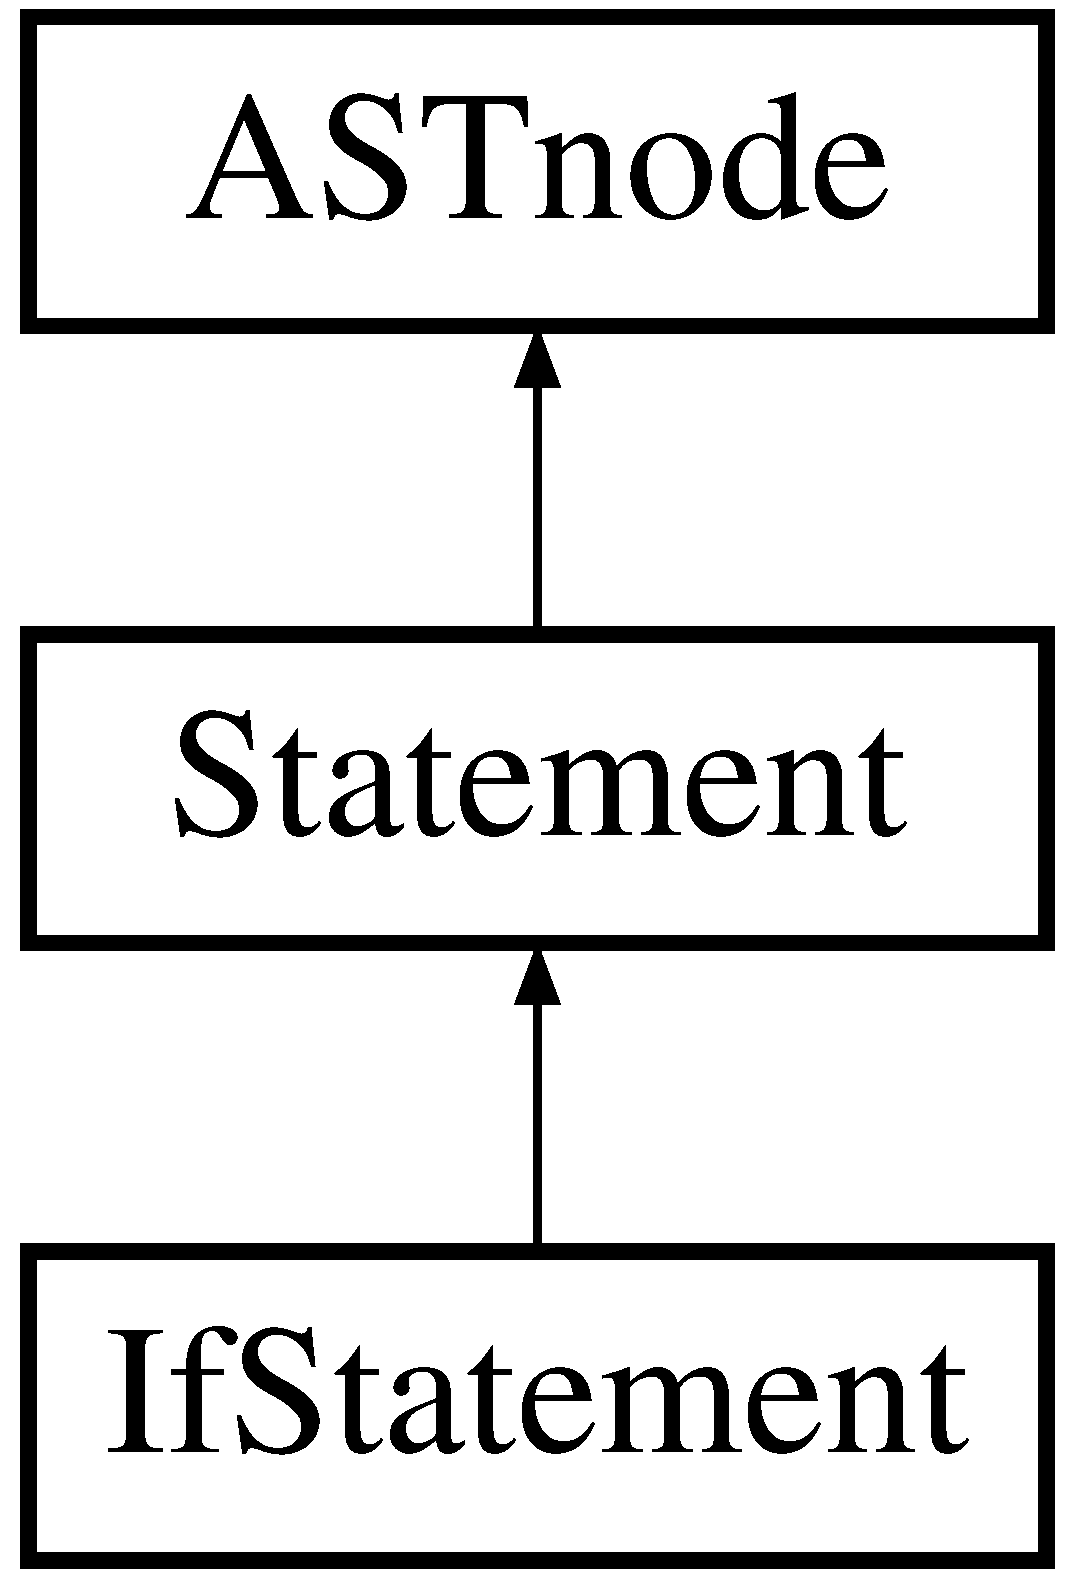
\includegraphics[height=3.000000cm]{class_if_statement}
\end{center}
\end{figure}
\subsection*{Public Member Functions}
\begin{DoxyCompactItemize}
\item 
\mbox{\Hypertarget{class_if_statement_acd21e3b7cf623247ddc4926ab342a92e}\label{class_if_statement_acd21e3b7cf623247ddc4926ab342a92e}} 
{\bfseries If\+Statement} (const \hyperlink{class_expression}{Expression} $\ast$cond\+\_\+in, \hyperlink{class_statement}{Statement} $\ast$true\+\_\+in)
\item 
\mbox{\Hypertarget{class_if_statement_a25238ee0d79d96c1c28a18cf8cd45396}\label{class_if_statement_a25238ee0d79d96c1c28a18cf8cd45396}} 
void {\bfseries print} () const override
\item 
\mbox{\Hypertarget{class_if_statement_ac9134843bef45dd40db3cf1f5a282923}\label{class_if_statement_ac9134843bef45dd40db3cf1f5a282923}} 
void {\bfseries compile} (\hyperlink{class_context}{Context} \&ctxt, unsigned int dest\+Loc) const override
\end{DoxyCompactItemize}
\subsection*{Public Attributes}
\begin{DoxyCompactItemize}
\item 
\mbox{\Hypertarget{class_if_statement_a67ece738b44b6d4abd5919193147872c}\label{class_if_statement_a67ece738b44b6d4abd5919193147872c}} 
const \hyperlink{class_expression}{Expression} $\ast$ {\bfseries condition}
\item 
\mbox{\Hypertarget{class_if_statement_a8c21d800142cba3f2845f19b47f51c67}\label{class_if_statement_a8c21d800142cba3f2845f19b47f51c67}} 
\hyperlink{class_statement}{Statement} $\ast$ {\bfseries trueclause}
\end{DoxyCompactItemize}


The documentation for this class was generated from the following files\+:\begin{DoxyCompactItemize}
\item 
ast.\+hpp\item 
ast.\+cpp\end{DoxyCompactItemize}

\hypertarget{structjson__obj}{}\section{json\+\_\+obj Struct Reference}
\label{structjson__obj}\index{json\+\_\+obj@{json\+\_\+obj}}
\subsection*{Public Member Functions}
\begin{DoxyCompactItemize}
\item 
\mbox{\Hypertarget{structjson__obj_ac060ccd9342d0907f45bc0d02a3889e0}\label{structjson__obj_ac060ccd9342d0907f45bc0d02a3889e0}} 
string {\bfseries to\+\_\+print} ()
\end{DoxyCompactItemize}
\subsection*{Public Attributes}
\begin{DoxyCompactItemize}
\item 
\mbox{\Hypertarget{structjson__obj_a1bab31ab3b593bd6bf6c7948a817c330}\label{structjson__obj_a1bab31ab3b593bd6bf6c7948a817c330}} 
string {\bfseries text} = \char`\"{}\char`\"{}
\item 
\mbox{\Hypertarget{structjson__obj_a9a34007fff15c94c9c868563d960fad2}\label{structjson__obj_a9a34007fff15c94c9c868563d960fad2}} 
string {\bfseries class\+\_\+} = \char`\"{}\char`\"{}
\item 
\mbox{\Hypertarget{structjson__obj_afedfe1b83d34118ac2e8cabcd76ae575}\label{structjson__obj_afedfe1b83d34118ac2e8cabcd76ae575}} 
int {\bfseries stream\+Line} = 0
\item 
\mbox{\Hypertarget{structjson__obj_ad391b9438655833d64eb608c946876ca}\label{structjson__obj_ad391b9438655833d64eb608c946876ca}} 
string {\bfseries source\+File} = \char`\"{}\char`\"{}
\item 
\mbox{\Hypertarget{structjson__obj_a17a2555d0f7accf0e9955ca75962e7bf}\label{structjson__obj_a17a2555d0f7accf0e9955ca75962e7bf}} 
int {\bfseries source\+Line} = 0
\item 
\mbox{\Hypertarget{structjson__obj_a62e4cdcb3c699df8b272644afb06c564}\label{structjson__obj_a62e4cdcb3c699df8b272644afb06c564}} 
int {\bfseries source\+Col} = 0
\end{DoxyCompactItemize}


The documentation for this struct was generated from the following file\+:\begin{DoxyCompactItemize}
\item 
c\+\_\+lexer.\+cpp\end{DoxyCompactItemize}

\hypertarget{class_param_dec}{}\section{Param\+Dec Class Reference}
\label{class_param_dec}\index{Param\+Dec@{Param\+Dec}}
Inheritance diagram for Param\+Dec\+:\begin{figure}[H]
\begin{center}
\leavevmode
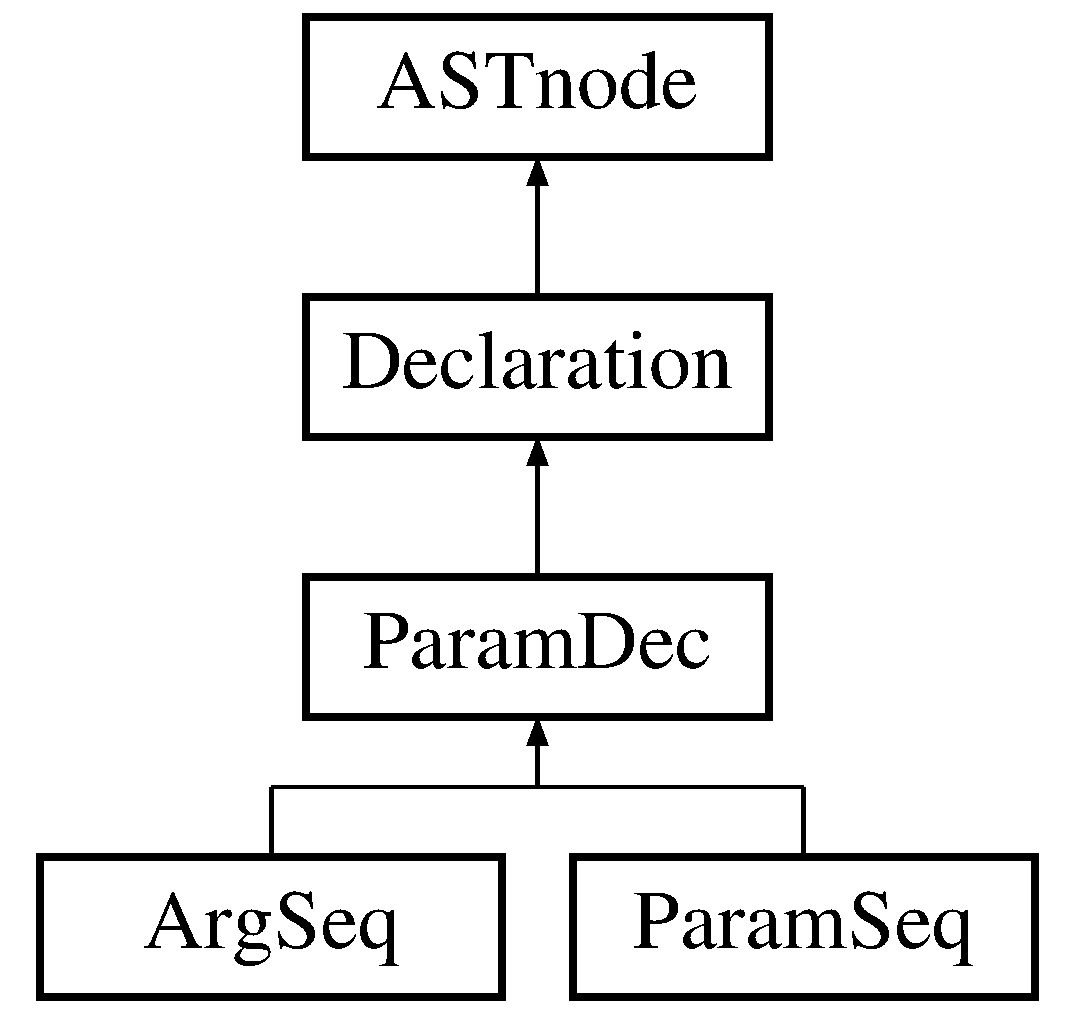
\includegraphics[height=4.000000cm]{class_param_dec}
\end{center}
\end{figure}
\subsection*{Public Member Functions}
\begin{DoxyCompactItemize}
\item 
\mbox{\Hypertarget{class_param_dec_a59a780182ef445ee791549918c5b5f04}\label{class_param_dec_a59a780182ef445ee791549918c5b5f04}} 
{\bfseries Param\+Dec} (const std\+::string $\ast$\+\_\+type, const std\+::string $\ast$\+\_\+id)
\item 
\mbox{\Hypertarget{class_param_dec_a0162a8316dc39022f906104a14e990cd}\label{class_param_dec_a0162a8316dc39022f906104a14e990cd}} 
{\bfseries Param\+Dec} (const \hyperlink{class_param_dec}{Param\+Dec} $\ast$p)
\item 
\mbox{\Hypertarget{class_param_dec_af2a5cf5fdd909c1c997ef54a55338375}\label{class_param_dec_af2a5cf5fdd909c1c997ef54a55338375}} 
void {\bfseries print} () const override
\item 
\mbox{\Hypertarget{class_param_dec_a85676e857de493242fad995d165f190f}\label{class_param_dec_a85676e857de493242fad995d165f190f}} 
void {\bfseries compile} (\hyperlink{class_context}{Context} \&ctxt, unsigned int dest\+Loc) const override
\end{DoxyCompactItemize}
\subsection*{Public Attributes}
\begin{DoxyCompactItemize}
\item 
\mbox{\Hypertarget{class_param_dec_a0a806710417048c81c274d4271e737e2}\label{class_param_dec_a0a806710417048c81c274d4271e737e2}} 
const std\+::string $\ast$ {\bfseries type}
\item 
\mbox{\Hypertarget{class_param_dec_a1fc979a07268fc208317f47fb7fbacf3}\label{class_param_dec_a1fc979a07268fc208317f47fb7fbacf3}} 
const std\+::string $\ast$ {\bfseries id}
\end{DoxyCompactItemize}


The documentation for this class was generated from the following files\+:\begin{DoxyCompactItemize}
\item 
ast.\+hpp\item 
ast.\+cpp\end{DoxyCompactItemize}

\hypertarget{class_param_seq}{}\section{Param\+Seq Class Reference}
\label{class_param_seq}\index{Param\+Seq@{Param\+Seq}}
Inheritance diagram for Param\+Seq\+:\begin{figure}[H]
\begin{center}
\leavevmode
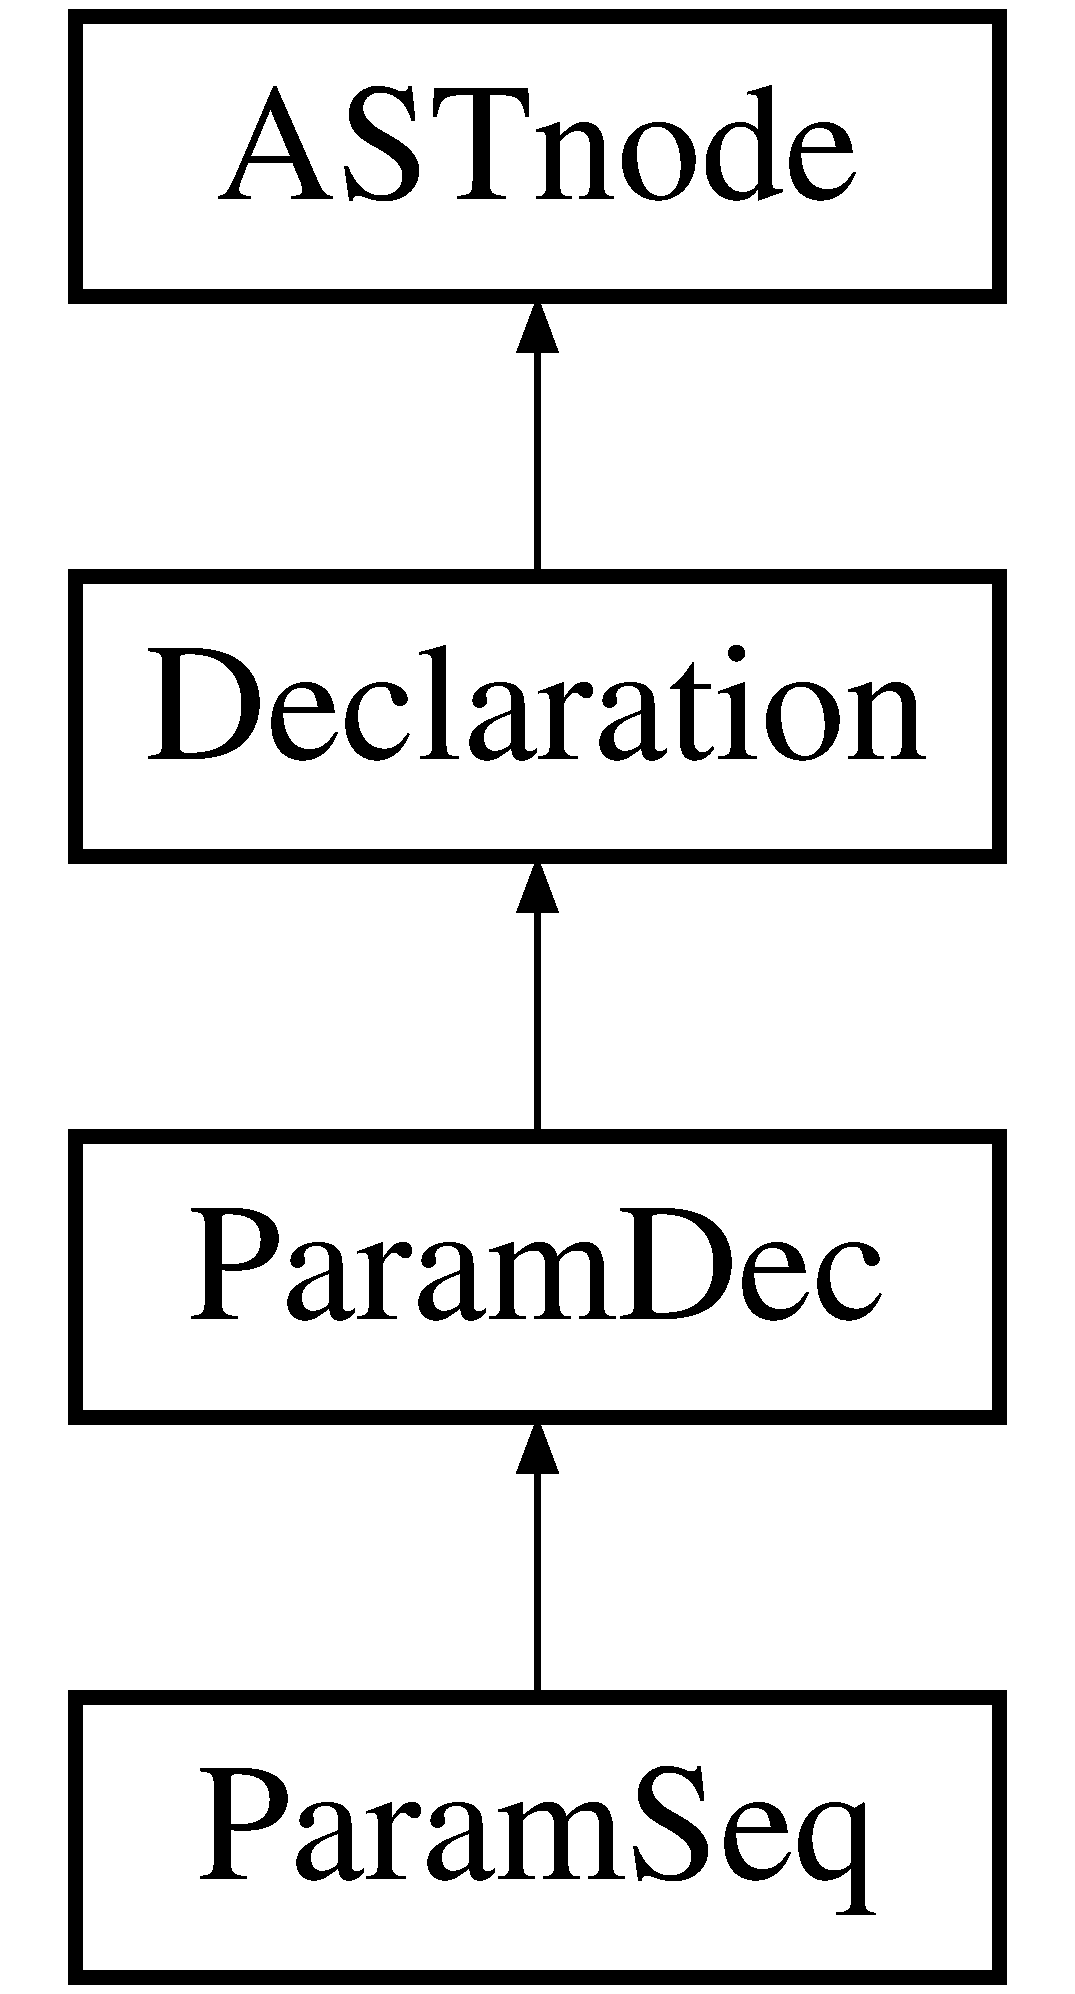
\includegraphics[height=4.000000cm]{class_param_seq}
\end{center}
\end{figure}
\subsection*{Public Member Functions}
\begin{DoxyCompactItemize}
\item 
\mbox{\Hypertarget{class_param_seq_a420d3b94a93ed350d3105d3a1f6ba6cb}\label{class_param_seq_a420d3b94a93ed350d3105d3a1f6ba6cb}} 
int {\bfseries get\+Count} () const
\item 
\mbox{\Hypertarget{class_param_seq_ae3f4fae87e4d53ec8b6562ddfc7c348b}\label{class_param_seq_ae3f4fae87e4d53ec8b6562ddfc7c348b}} 
const \hyperlink{class_param_dec}{Param\+Dec} $\ast$ {\bfseries get\+Declaration} (unsigned int i) const
\item 
\mbox{\Hypertarget{class_param_seq_a873e0fbdd7b78c81c8ca1a6534025c68}\label{class_param_seq_a873e0fbdd7b78c81c8ca1a6534025c68}} 
void {\bfseries add\+Declaration} (\hyperlink{class_param_dec}{Param\+Dec} $\ast$state)
\item 
\mbox{\Hypertarget{class_param_seq_af48a90dce132044d38173108734cb2b4}\label{class_param_seq_af48a90dce132044d38173108734cb2b4}} 
void {\bfseries print} () const override
\item 
\mbox{\Hypertarget{class_param_seq_a696b80ee646bee48d67755cb2e20d77f}\label{class_param_seq_a696b80ee646bee48d67755cb2e20d77f}} 
void {\bfseries compile} (\hyperlink{class_context}{Context} \&ctxt, unsigned int dest\+Loc) const override
\end{DoxyCompactItemize}
\subsection*{Additional Inherited Members}


The documentation for this class was generated from the following files\+:\begin{DoxyCompactItemize}
\item 
ast.\+hpp\item 
ast.\+cpp\end{DoxyCompactItemize}

\hypertarget{class_program}{}\section{Program Class Reference}
\label{class_program}\index{Program@{Program}}
Inheritance diagram for Program\+:\begin{figure}[H]
\begin{center}
\leavevmode
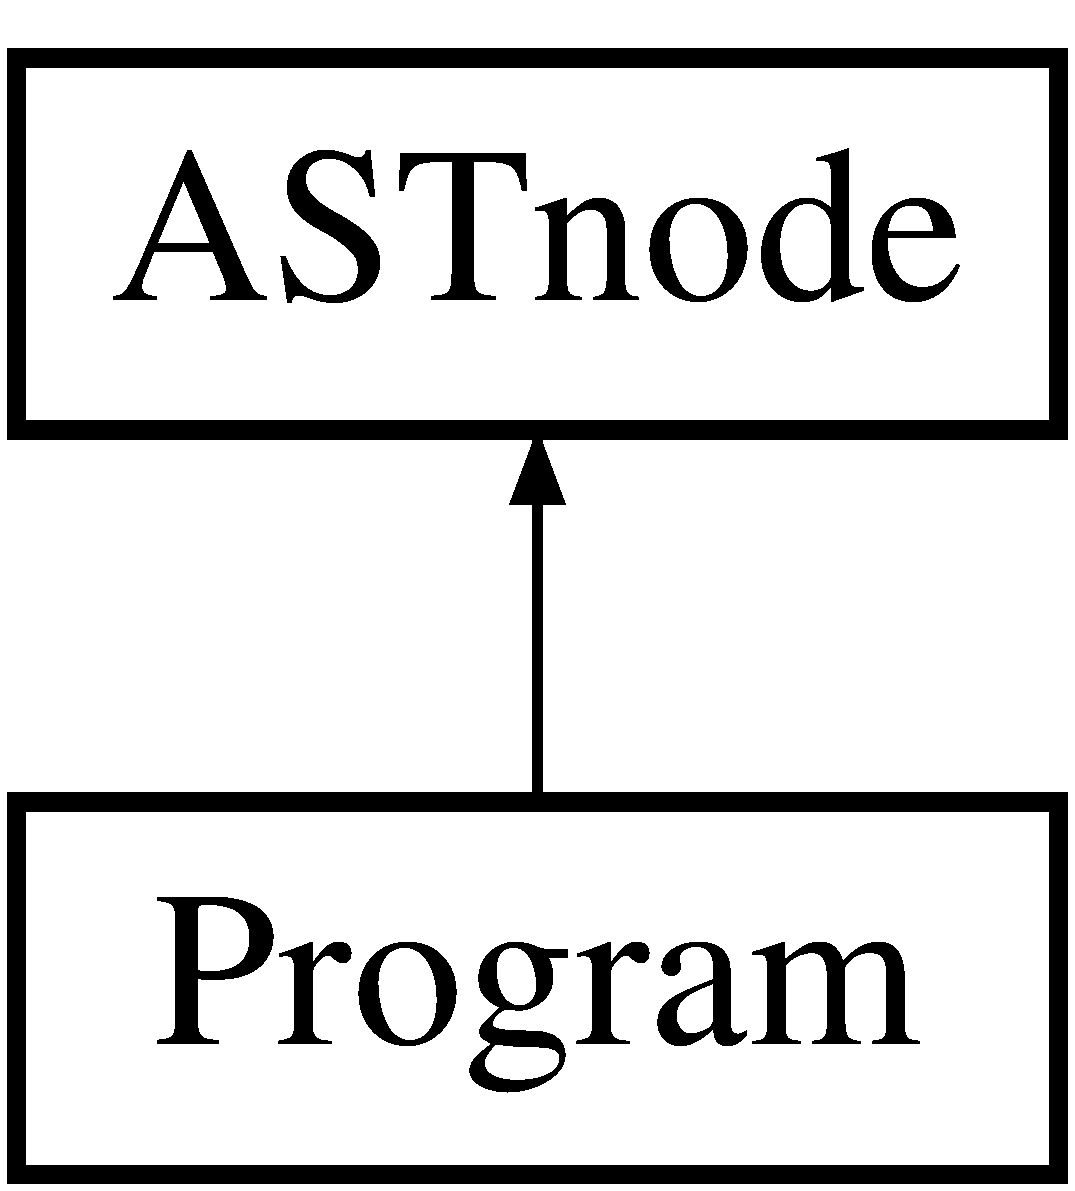
\includegraphics[height=2.000000cm]{class_program}
\end{center}
\end{figure}
\subsection*{Public Member Functions}
\begin{DoxyCompactItemize}
\item 
\mbox{\Hypertarget{class_program_a9a5473625b89733ce60dd52ad61a550a}\label{class_program_a9a5473625b89733ce60dd52ad61a550a}} 
{\bfseries Program} (const \hyperlink{class_a_s_tnode}{A\+S\+Tnode} $\ast$left\+\_\+in)
\item 
\mbox{\Hypertarget{class_program_a1a53dfe912e66b455561c83100c6613b}\label{class_program_a1a53dfe912e66b455561c83100c6613b}} 
{\bfseries Program} (const \hyperlink{class_a_s_tnode}{A\+S\+Tnode} $\ast$left\+\_\+in, const \hyperlink{class_a_s_tnode}{A\+S\+Tnode} $\ast$right\+\_\+in)
\item 
\mbox{\Hypertarget{class_program_a47be112193d16addb2d5c6d11df28226}\label{class_program_a47be112193d16addb2d5c6d11df28226}} 
void {\bfseries print} () const override
\item 
\mbox{\Hypertarget{class_program_ac7ff0e76139a2c2b93add868d4fe5cda}\label{class_program_ac7ff0e76139a2c2b93add868d4fe5cda}} 
void {\bfseries compile} (\hyperlink{class_context}{Context} \&ctxt, unsigned int dest\+Loc) const override
\end{DoxyCompactItemize}
\subsection*{Public Attributes}
\begin{DoxyCompactItemize}
\item 
\mbox{\Hypertarget{class_program_a993a98af530d1922338cbc49e6bc83d5}\label{class_program_a993a98af530d1922338cbc49e6bc83d5}} 
const \hyperlink{class_a_s_tnode}{A\+S\+Tnode} $\ast$ {\bfseries left}
\item 
\mbox{\Hypertarget{class_program_ac9e819c11146c9ad247ddd9bac53c0ff}\label{class_program_ac9e819c11146c9ad247ddd9bac53c0ff}} 
const \hyperlink{class_a_s_tnode}{A\+S\+Tnode} $\ast$ {\bfseries right}
\end{DoxyCompactItemize}


The documentation for this class was generated from the following files\+:\begin{DoxyCompactItemize}
\item 
ast.\+hpp\item 
ast.\+cpp\end{DoxyCompactItemize}

\hypertarget{class_return_statement}{}\section{Return\+Statement Class Reference}
\label{class_return_statement}\index{Return\+Statement@{Return\+Statement}}
Inheritance diagram for Return\+Statement\+:\begin{figure}[H]
\begin{center}
\leavevmode
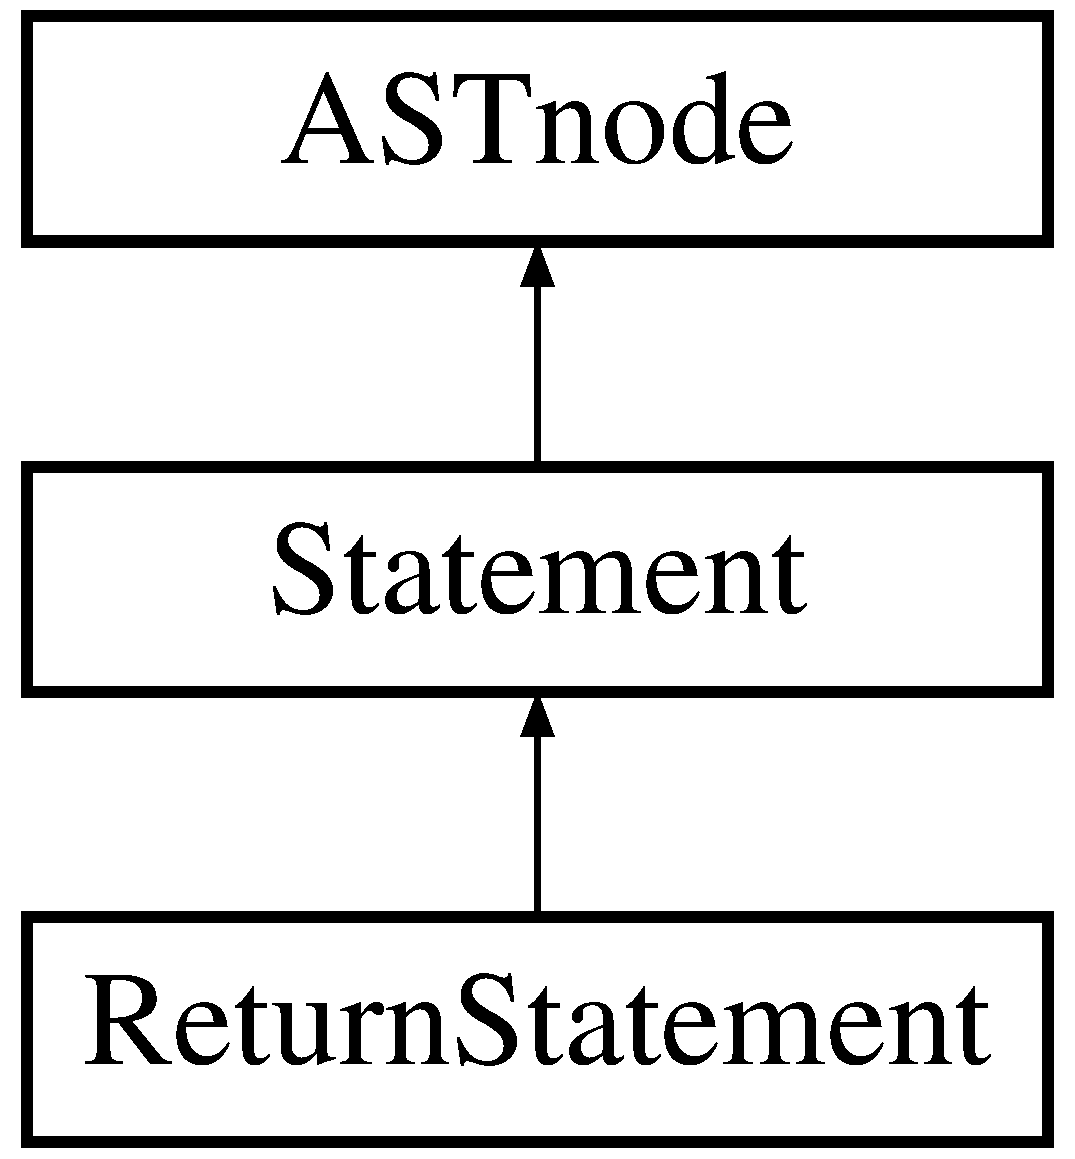
\includegraphics[height=3.000000cm]{class_return_statement}
\end{center}
\end{figure}
\subsection*{Public Member Functions}
\begin{DoxyCompactItemize}
\item 
\mbox{\Hypertarget{class_return_statement_afa9044bef48163f409d0910cab7aad21}\label{class_return_statement_afa9044bef48163f409d0910cab7aad21}} 
{\bfseries Return\+Statement} (const \hyperlink{class_expression}{Expression} $\ast$in)
\item 
\mbox{\Hypertarget{class_return_statement_a90e892fc6a685a31f3251946ab02348b}\label{class_return_statement_a90e892fc6a685a31f3251946ab02348b}} 
void {\bfseries print} () const override
\item 
\mbox{\Hypertarget{class_return_statement_aad7f97ab1984c0da326157d6b06b162f}\label{class_return_statement_aad7f97ab1984c0da326157d6b06b162f}} 
void {\bfseries compile} (\hyperlink{class_context}{Context} \&ctxt, unsigned int dest\+Loc) const override
\end{DoxyCompactItemize}
\subsection*{Public Attributes}
\begin{DoxyCompactItemize}
\item 
\mbox{\Hypertarget{class_return_statement_a1ecfd5e94a511544e9dd4fbdfa81ea4a}\label{class_return_statement_a1ecfd5e94a511544e9dd4fbdfa81ea4a}} 
const \hyperlink{class_expression}{Expression} $\ast$ {\bfseries thing}
\end{DoxyCompactItemize}


The documentation for this class was generated from the following files\+:\begin{DoxyCompactItemize}
\item 
ast.\+hpp\item 
ast.\+cpp\end{DoxyCompactItemize}

\hypertarget{class_scope}{}\section{Scope Class Reference}
\label{class_scope}\index{Scope@{Scope}}
Inheritance diagram for Scope\+:\begin{figure}[H]
\begin{center}
\leavevmode
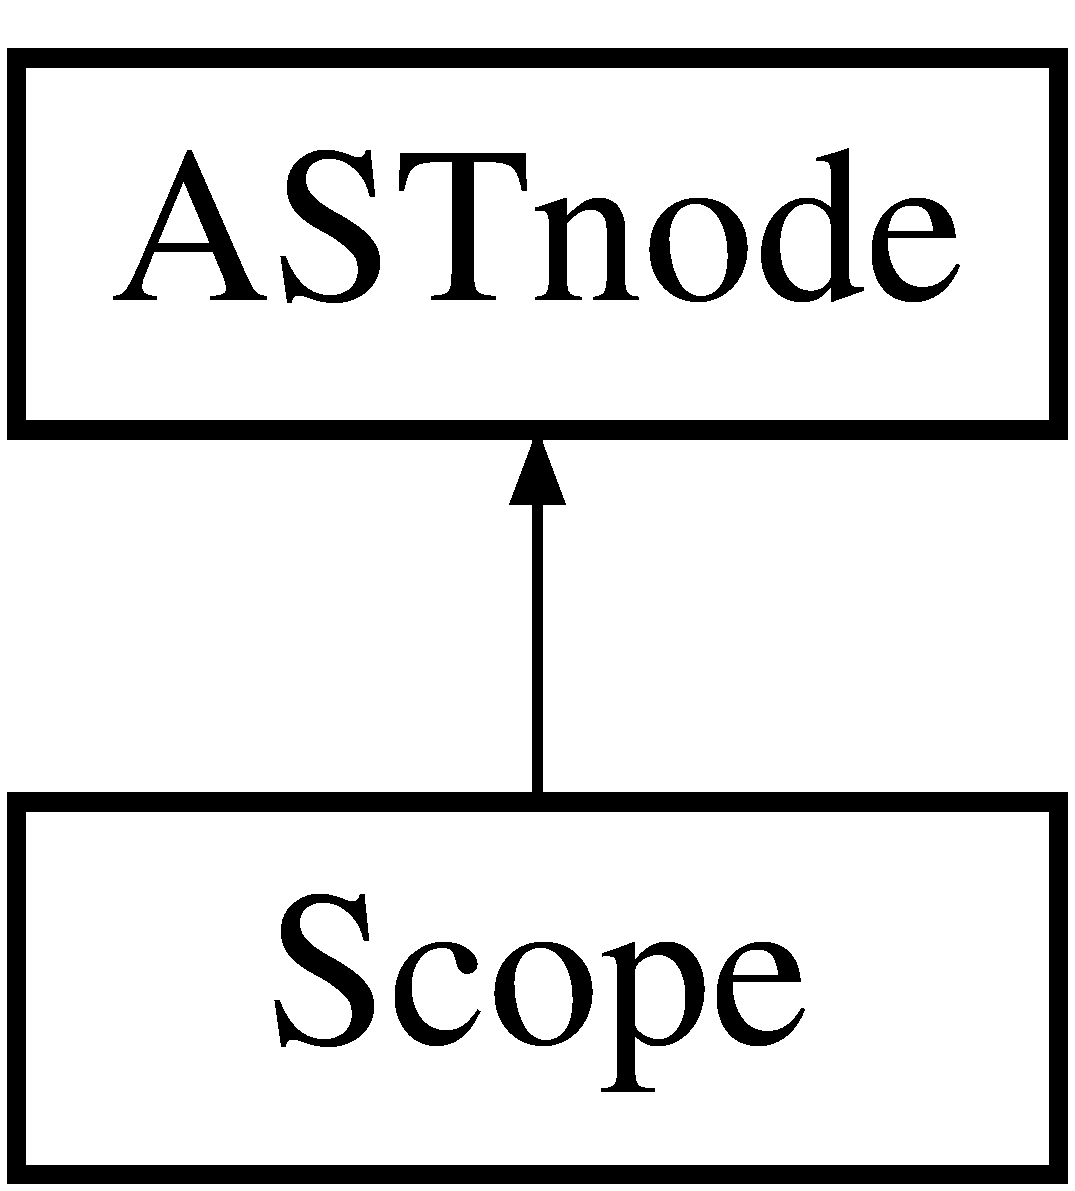
\includegraphics[height=2.000000cm]{class_scope}
\end{center}
\end{figure}
\subsection*{Public Member Functions}
\begin{DoxyCompactItemize}
\item 
\mbox{\Hypertarget{class_scope_a78f67e3251df41af3095bbf6b0716624}\label{class_scope_a78f67e3251df41af3095bbf6b0716624}} 
{\bfseries Scope} (\hyperlink{class_var_seq}{Var\+Seq} $\ast$decls\+\_\+in)
\item 
\mbox{\Hypertarget{class_scope_af2f563a3fd5083aa4f623960a3b26055}\label{class_scope_af2f563a3fd5083aa4f623960a3b26055}} 
{\bfseries Scope} (\hyperlink{class_statement_sequence}{Statement\+Sequence} $\ast$stats\+\_\+in)
\item 
\mbox{\Hypertarget{class_scope_a3a7352ed3324dc4a3f2073eb70fa0b92}\label{class_scope_a3a7352ed3324dc4a3f2073eb70fa0b92}} 
{\bfseries Scope} (\hyperlink{class_var_seq}{Var\+Seq} $\ast$decls\+\_\+in, \hyperlink{class_statement_sequence}{Statement\+Sequence} $\ast$stats\+\_\+in)
\item 
\mbox{\Hypertarget{class_scope_acf0c61b1ea1225a47975aa2ab3ed195d}\label{class_scope_acf0c61b1ea1225a47975aa2ab3ed195d}} 
void {\bfseries print} () const override
\item 
\mbox{\Hypertarget{class_scope_ab860a2c5e545bbc689aca48b8582971b}\label{class_scope_ab860a2c5e545bbc689aca48b8582971b}} 
void {\bfseries compile} (\hyperlink{class_context}{Context} \&ctxt, unsigned int dest\+Loc) const override
\end{DoxyCompactItemize}
\subsection*{Public Attributes}
\begin{DoxyCompactItemize}
\item 
\mbox{\Hypertarget{class_scope_ad26ebfb097bd2407e12844ec97ec6dd3}\label{class_scope_ad26ebfb097bd2407e12844ec97ec6dd3}} 
\hyperlink{class_var_seq}{Var\+Seq} $\ast$ {\bfseries decls}
\item 
\mbox{\Hypertarget{class_scope_a7c881cb6c8283bd257b33d698ffd9a99}\label{class_scope_a7c881cb6c8283bd257b33d698ffd9a99}} 
\hyperlink{class_statement_sequence}{Statement\+Sequence} $\ast$ {\bfseries stats}
\end{DoxyCompactItemize}


The documentation for this class was generated from the following files\+:\begin{DoxyCompactItemize}
\item 
ast.\+hpp\item 
ast.\+cpp\end{DoxyCompactItemize}

\hypertarget{class_scope_statement}{}\section{Scope\+Statement Class Reference}
\label{class_scope_statement}\index{Scope\+Statement@{Scope\+Statement}}
Inheritance diagram for Scope\+Statement\+:\begin{figure}[H]
\begin{center}
\leavevmode
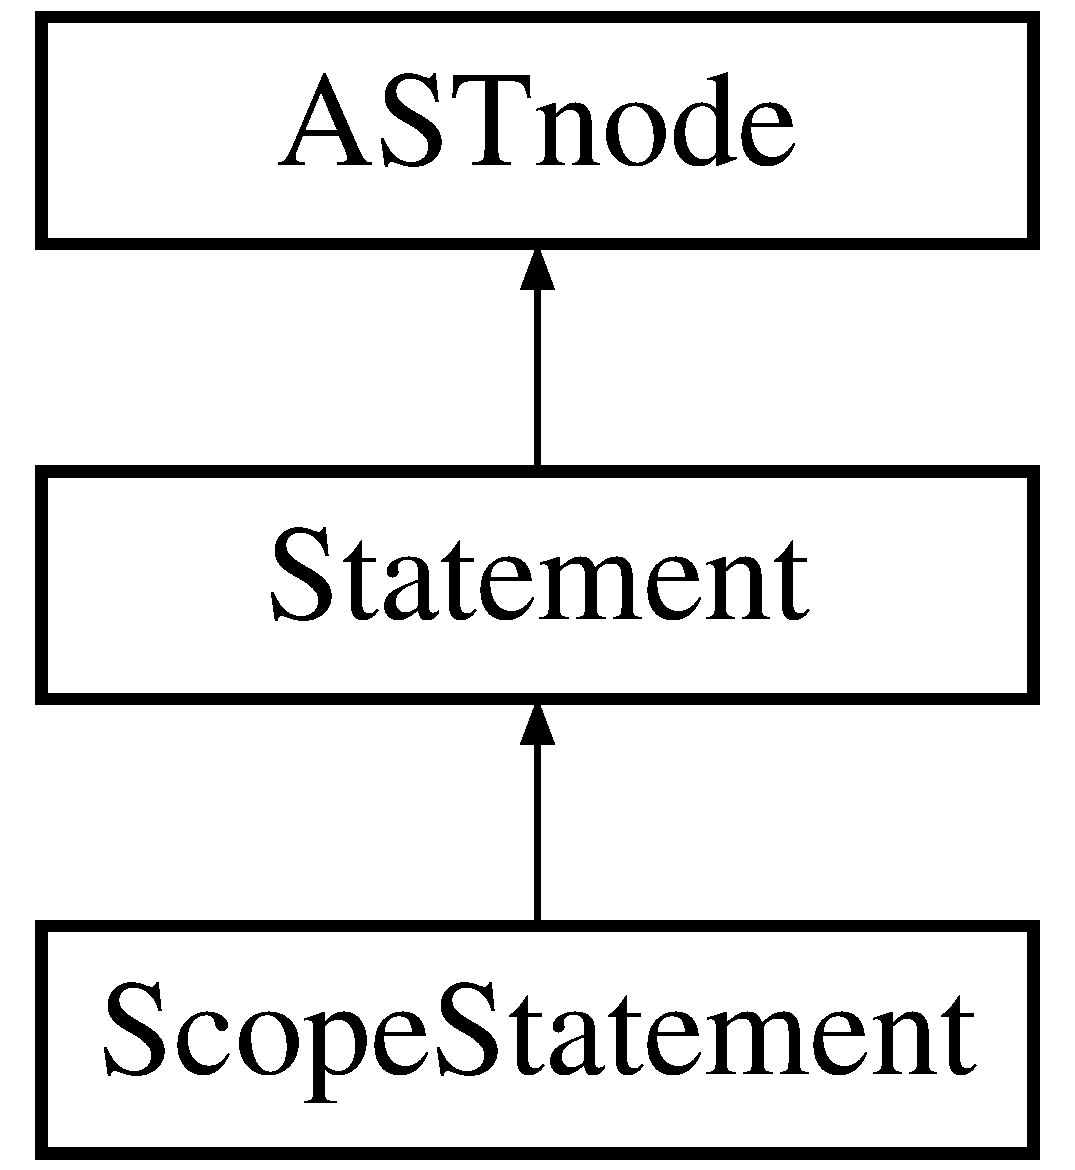
\includegraphics[height=3.000000cm]{class_scope_statement}
\end{center}
\end{figure}
\subsection*{Public Member Functions}
\begin{DoxyCompactItemize}
\item 
\mbox{\Hypertarget{class_scope_statement_a17c2b8bba07c5042b948468813df0598}\label{class_scope_statement_a17c2b8bba07c5042b948468813df0598}} 
{\bfseries Scope\+Statement} (const \hyperlink{class_scope}{Scope} $\ast$scope)
\item 
\mbox{\Hypertarget{class_scope_statement_ac18275b37ae4396ffbcda7ee03794ba1}\label{class_scope_statement_ac18275b37ae4396ffbcda7ee03794ba1}} 
void {\bfseries print} () const override
\item 
\mbox{\Hypertarget{class_scope_statement_a3536a9dd302b5dc617cdd4bab7fe91ce}\label{class_scope_statement_a3536a9dd302b5dc617cdd4bab7fe91ce}} 
void {\bfseries compile} (\hyperlink{class_context}{Context} \&ctxt, unsigned int dest\+Loc) const override
\end{DoxyCompactItemize}
\subsection*{Public Attributes}
\begin{DoxyCompactItemize}
\item 
\mbox{\Hypertarget{class_scope_statement_ad0f3bd2bc12e604f176d7e9046a5ec79}\label{class_scope_statement_ad0f3bd2bc12e604f176d7e9046a5ec79}} 
const \hyperlink{class_scope}{Scope} $\ast$ {\bfseries scope}
\end{DoxyCompactItemize}


The documentation for this class was generated from the following files\+:\begin{DoxyCompactItemize}
\item 
ast.\+hpp\item 
ast.\+cpp\end{DoxyCompactItemize}

\hypertarget{class_statement}{}\section{Statement Class Reference}
\label{class_statement}\index{Statement@{Statement}}
Inheritance diagram for Statement\+:\begin{figure}[H]
\begin{center}
\leavevmode
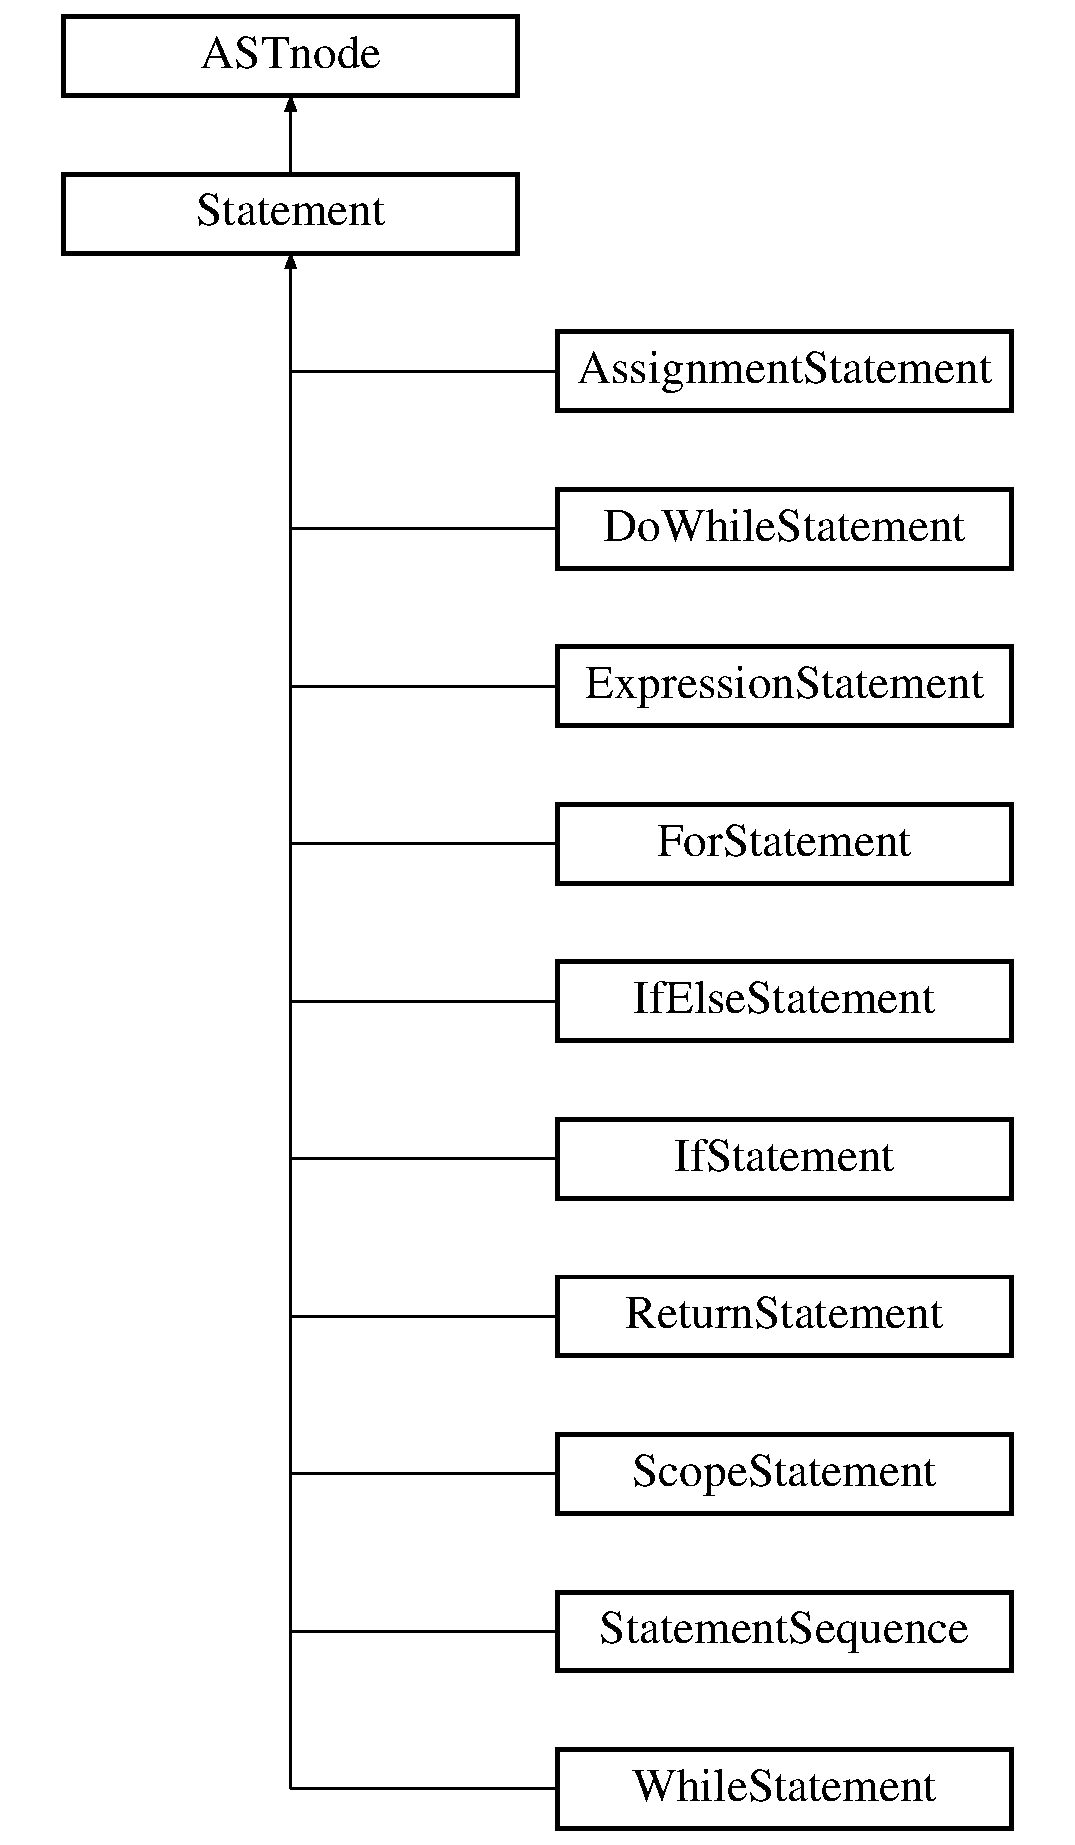
\includegraphics[height=12.000000cm]{class_statement}
\end{center}
\end{figure}
\subsection*{Public Member Functions}
\begin{DoxyCompactItemize}
\item 
\mbox{\Hypertarget{class_statement_a22fdc19952a84e649e0540abfdb704a0}\label{class_statement_a22fdc19952a84e649e0540abfdb704a0}} 
virtual void {\bfseries print} () const =0
\item 
\mbox{\Hypertarget{class_statement_a9ac6b523a651324555cd3fd1dac322fc}\label{class_statement_a9ac6b523a651324555cd3fd1dac322fc}} 
virtual void {\bfseries compile} (\hyperlink{class_context}{Context} \&ctxt, unsigned int dest\+Loc) const =0
\end{DoxyCompactItemize}


The documentation for this class was generated from the following file\+:\begin{DoxyCompactItemize}
\item 
ast.\+hpp\end{DoxyCompactItemize}

\hypertarget{class_statement_sequence}{}\section{Statement\+Sequence Class Reference}
\label{class_statement_sequence}\index{Statement\+Sequence@{Statement\+Sequence}}
Inheritance diagram for Statement\+Sequence\+:\begin{figure}[H]
\begin{center}
\leavevmode
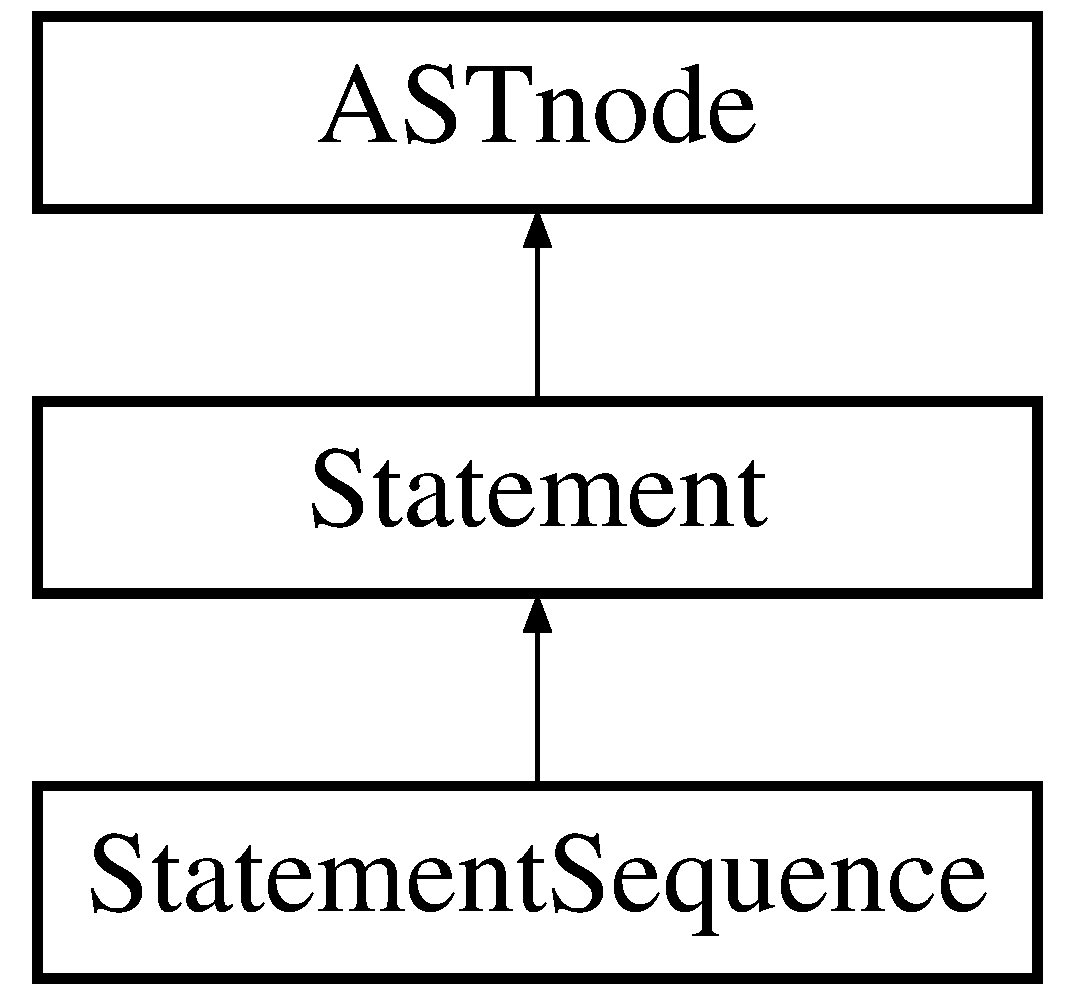
\includegraphics[height=3.000000cm]{class_statement_sequence}
\end{center}
\end{figure}
\subsection*{Public Member Functions}
\begin{DoxyCompactItemize}
\item 
\mbox{\Hypertarget{class_statement_sequence_aabfb1f6393ce14ed25da26a9bf4bc0a1}\label{class_statement_sequence_aabfb1f6393ce14ed25da26a9bf4bc0a1}} 
int {\bfseries get\+Count} () const
\item 
\mbox{\Hypertarget{class_statement_sequence_abc55c98ec4555f7c8c9c3a05c7acd65b}\label{class_statement_sequence_abc55c98ec4555f7c8c9c3a05c7acd65b}} 
const \hyperlink{class_statement}{Statement} $\ast$ {\bfseries get\+Statement} (unsigned int i) const
\item 
\mbox{\Hypertarget{class_statement_sequence_a226f128693fd1ac1209dd3b4c0a36c5d}\label{class_statement_sequence_a226f128693fd1ac1209dd3b4c0a36c5d}} 
void {\bfseries add\+Statement} (\hyperlink{class_statement}{Statement} $\ast$state)
\item 
\mbox{\Hypertarget{class_statement_sequence_a26676a17f25d1f746d7246a846c7c484}\label{class_statement_sequence_a26676a17f25d1f746d7246a846c7c484}} 
void {\bfseries print} () const override
\item 
\mbox{\Hypertarget{class_statement_sequence_a514173eedcad219da4755f9b9185af16}\label{class_statement_sequence_a514173eedcad219da4755f9b9185af16}} 
void {\bfseries compile} (\hyperlink{class_context}{Context} \&ctxt, unsigned int dest\+Loc) const override
\end{DoxyCompactItemize}


The documentation for this class was generated from the following files\+:\begin{DoxyCompactItemize}
\item 
ast.\+hpp\item 
ast.\+cpp\end{DoxyCompactItemize}

\hypertarget{class_unary_expression}{}\section{Unary\+Expression Class Reference}
\label{class_unary_expression}\index{Unary\+Expression@{Unary\+Expression}}
Inheritance diagram for Unary\+Expression\+:\begin{figure}[H]
\begin{center}
\leavevmode
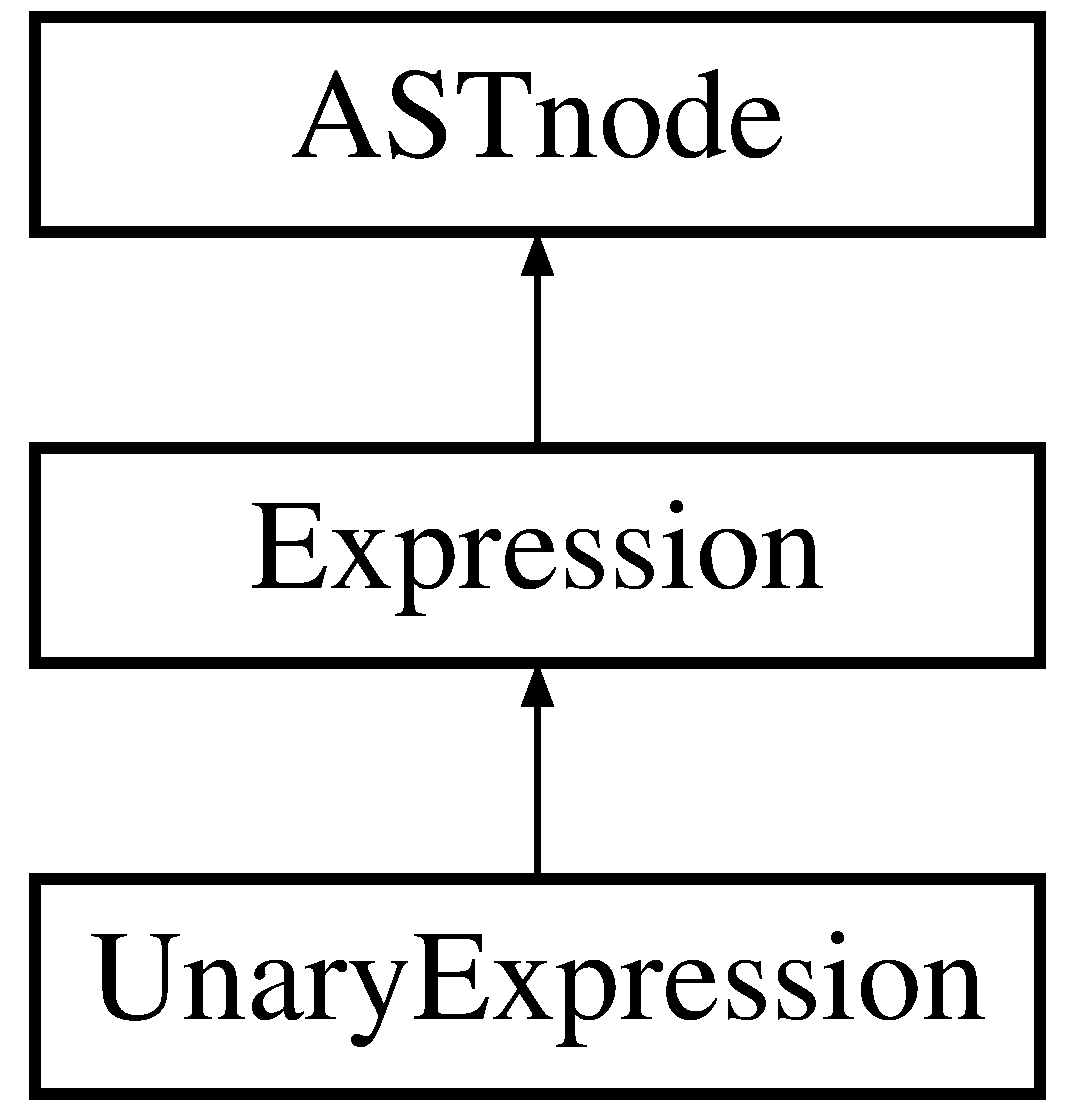
\includegraphics[height=3.000000cm]{class_unary_expression}
\end{center}
\end{figure}
\subsection*{Public Member Functions}
\begin{DoxyCompactItemize}
\item 
\mbox{\Hypertarget{class_unary_expression_aa28ae8e45294dbc001a2130cc034d3dd}\label{class_unary_expression_aa28ae8e45294dbc001a2130cc034d3dd}} 
{\bfseries Unary\+Expression} (const std\+::string $\ast$id\+\_\+in, const std\+::string $\ast$op\+\_\+in)
\item 
\mbox{\Hypertarget{class_unary_expression_afa622c4aa468c5b9b109ce0b56208fcb}\label{class_unary_expression_afa622c4aa468c5b9b109ce0b56208fcb}} 
void {\bfseries print} () const override
\item 
\mbox{\Hypertarget{class_unary_expression_af037b3b99f641a8594b5071a7ec23327}\label{class_unary_expression_af037b3b99f641a8594b5071a7ec23327}} 
void {\bfseries compile} (\hyperlink{class_context}{Context} \&ctxt, unsigned int dest\+Loc) const override
\end{DoxyCompactItemize}
\subsection*{Public Attributes}
\begin{DoxyCompactItemize}
\item 
\mbox{\Hypertarget{class_unary_expression_a3d0c1fd7b88bdcaafa8621fbc16d13f8}\label{class_unary_expression_a3d0c1fd7b88bdcaafa8621fbc16d13f8}} 
const std\+::string $\ast$ {\bfseries id}
\item 
\mbox{\Hypertarget{class_unary_expression_a10f6d008a699e30220e3778146e4ba22}\label{class_unary_expression_a10f6d008a699e30220e3778146e4ba22}} 
const std\+::string $\ast$ {\bfseries op}
\end{DoxyCompactItemize}


The documentation for this class was generated from the following files\+:\begin{DoxyCompactItemize}
\item 
ast.\+hpp\item 
ast.\+cpp\end{DoxyCompactItemize}

\hypertarget{class_var_dec}{}\section{Var\+Dec Class Reference}
\label{class_var_dec}\index{Var\+Dec@{Var\+Dec}}
Inheritance diagram for Var\+Dec\+:\begin{figure}[H]
\begin{center}
\leavevmode
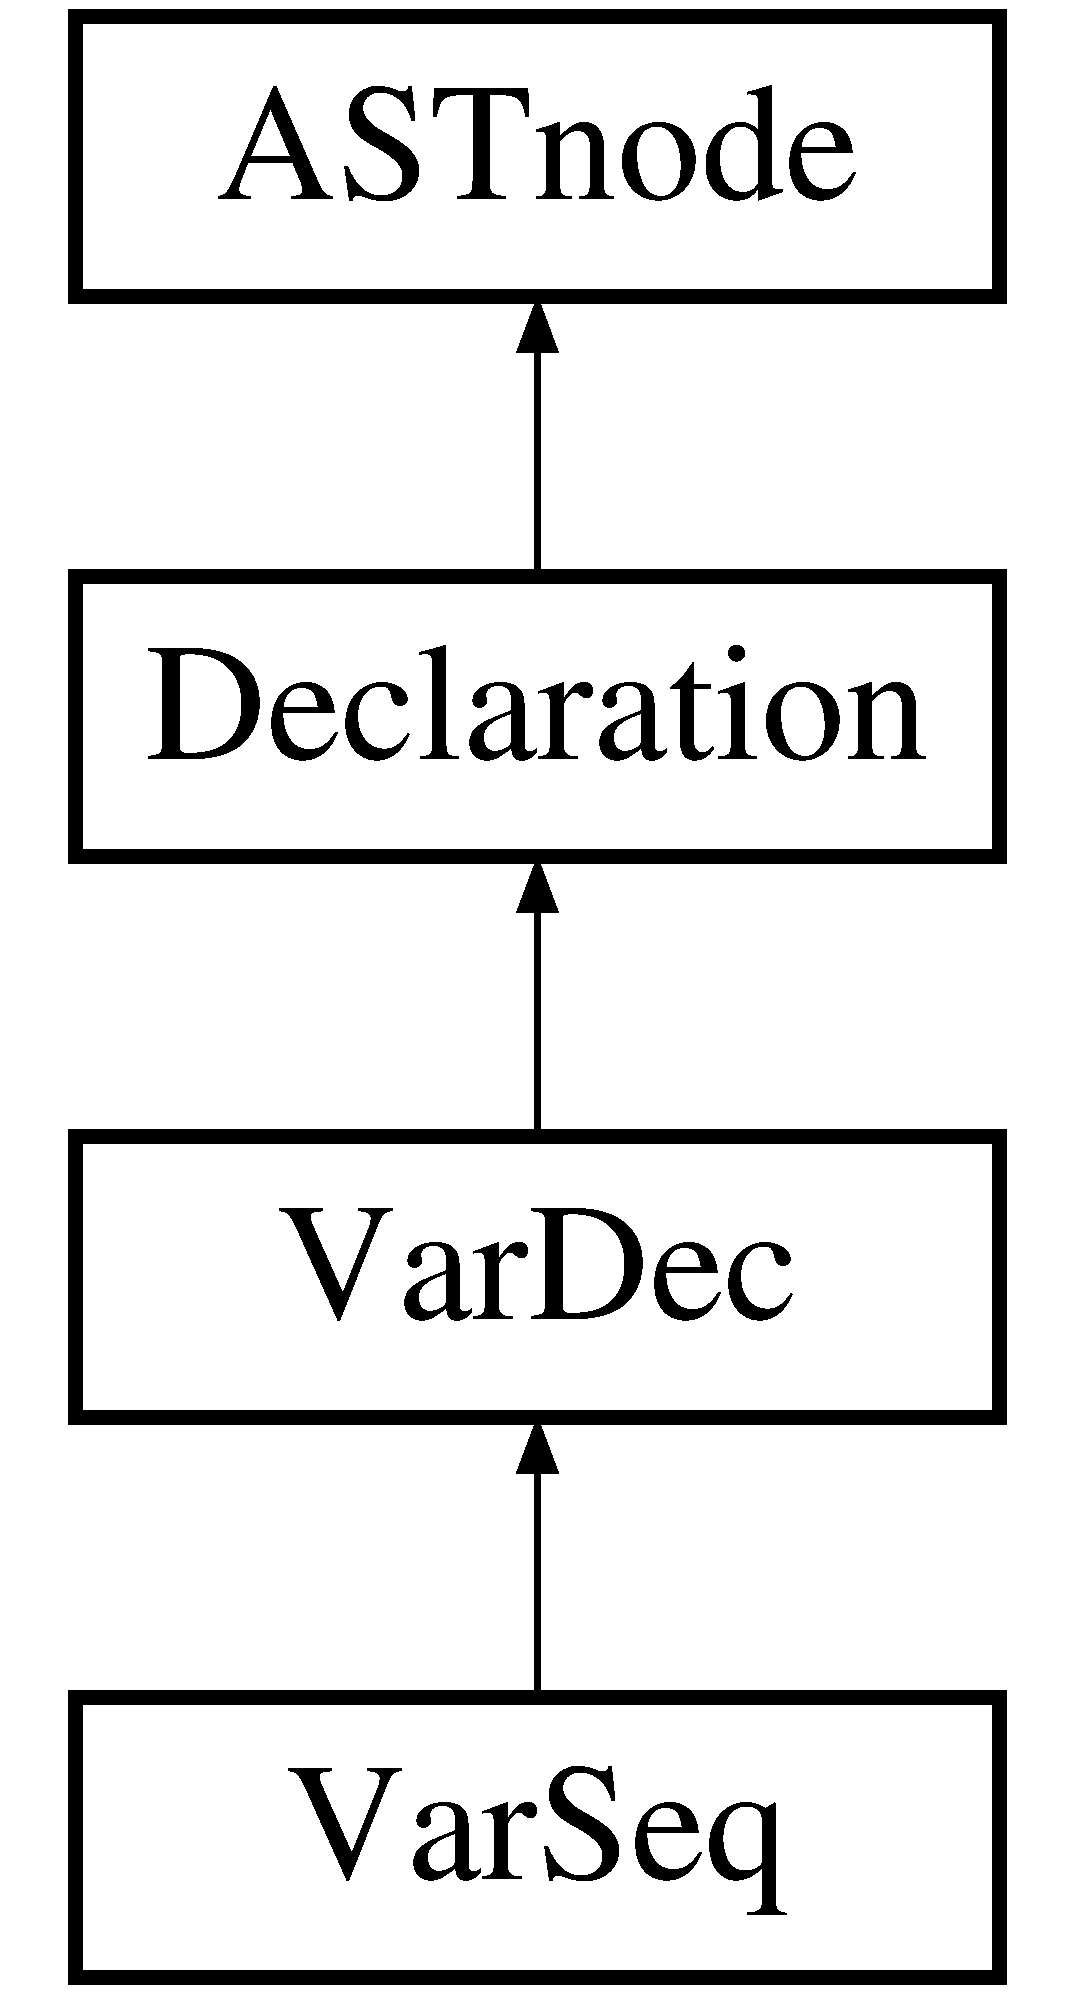
\includegraphics[height=4.000000cm]{class_var_dec}
\end{center}
\end{figure}
\subsection*{Public Member Functions}
\begin{DoxyCompactItemize}
\item 
\mbox{\Hypertarget{class_var_dec_a913d077202a7809a95e0b3ae304c2777}\label{class_var_dec_a913d077202a7809a95e0b3ae304c2777}} 
{\bfseries Var\+Dec} (const std\+::string $\ast$\+\_\+type, const std\+::string $\ast$\+\_\+id, const \hyperlink{class_expression}{Expression} $\ast$\+\_\+rhs)
\item 
\mbox{\Hypertarget{class_var_dec_ad0092f8b9f943682a3700013c707a8aa}\label{class_var_dec_ad0092f8b9f943682a3700013c707a8aa}} 
{\bfseries Var\+Dec} (const \hyperlink{class_var_dec}{Var\+Dec} $\ast$p)
\item 
\mbox{\Hypertarget{class_var_dec_ab4b9ec0d11e8cf7f8f16320ab8c6412c}\label{class_var_dec_ab4b9ec0d11e8cf7f8f16320ab8c6412c}} 
void {\bfseries print} () const override
\item 
\mbox{\Hypertarget{class_var_dec_a644242ce654fa31b8a97eebc7d7ef3e1}\label{class_var_dec_a644242ce654fa31b8a97eebc7d7ef3e1}} 
void {\bfseries compile} (\hyperlink{class_context}{Context} \&ctxt, unsigned int dest\+Loc) const override
\end{DoxyCompactItemize}
\subsection*{Public Attributes}
\begin{DoxyCompactItemize}
\item 
\mbox{\Hypertarget{class_var_dec_a389a60f027a4359d27fe550cd30bad4e}\label{class_var_dec_a389a60f027a4359d27fe550cd30bad4e}} 
const std\+::string $\ast$ {\bfseries type}
\item 
\mbox{\Hypertarget{class_var_dec_a5907906a3dff56774adf2f9d2822fd9a}\label{class_var_dec_a5907906a3dff56774adf2f9d2822fd9a}} 
const std\+::string $\ast$ {\bfseries id}
\item 
\mbox{\Hypertarget{class_var_dec_afce3b9ef23092a1aab5a649df5c1ee5b}\label{class_var_dec_afce3b9ef23092a1aab5a649df5c1ee5b}} 
const \hyperlink{class_expression}{Expression} $\ast$ {\bfseries rhs}
\end{DoxyCompactItemize}


The documentation for this class was generated from the following files\+:\begin{DoxyCompactItemize}
\item 
ast.\+hpp\item 
ast.\+cpp\end{DoxyCompactItemize}

\hypertarget{class_var_seq}{}\section{Var\+Seq Class Reference}
\label{class_var_seq}\index{Var\+Seq@{Var\+Seq}}
Inheritance diagram for Var\+Seq\+:\begin{figure}[H]
\begin{center}
\leavevmode
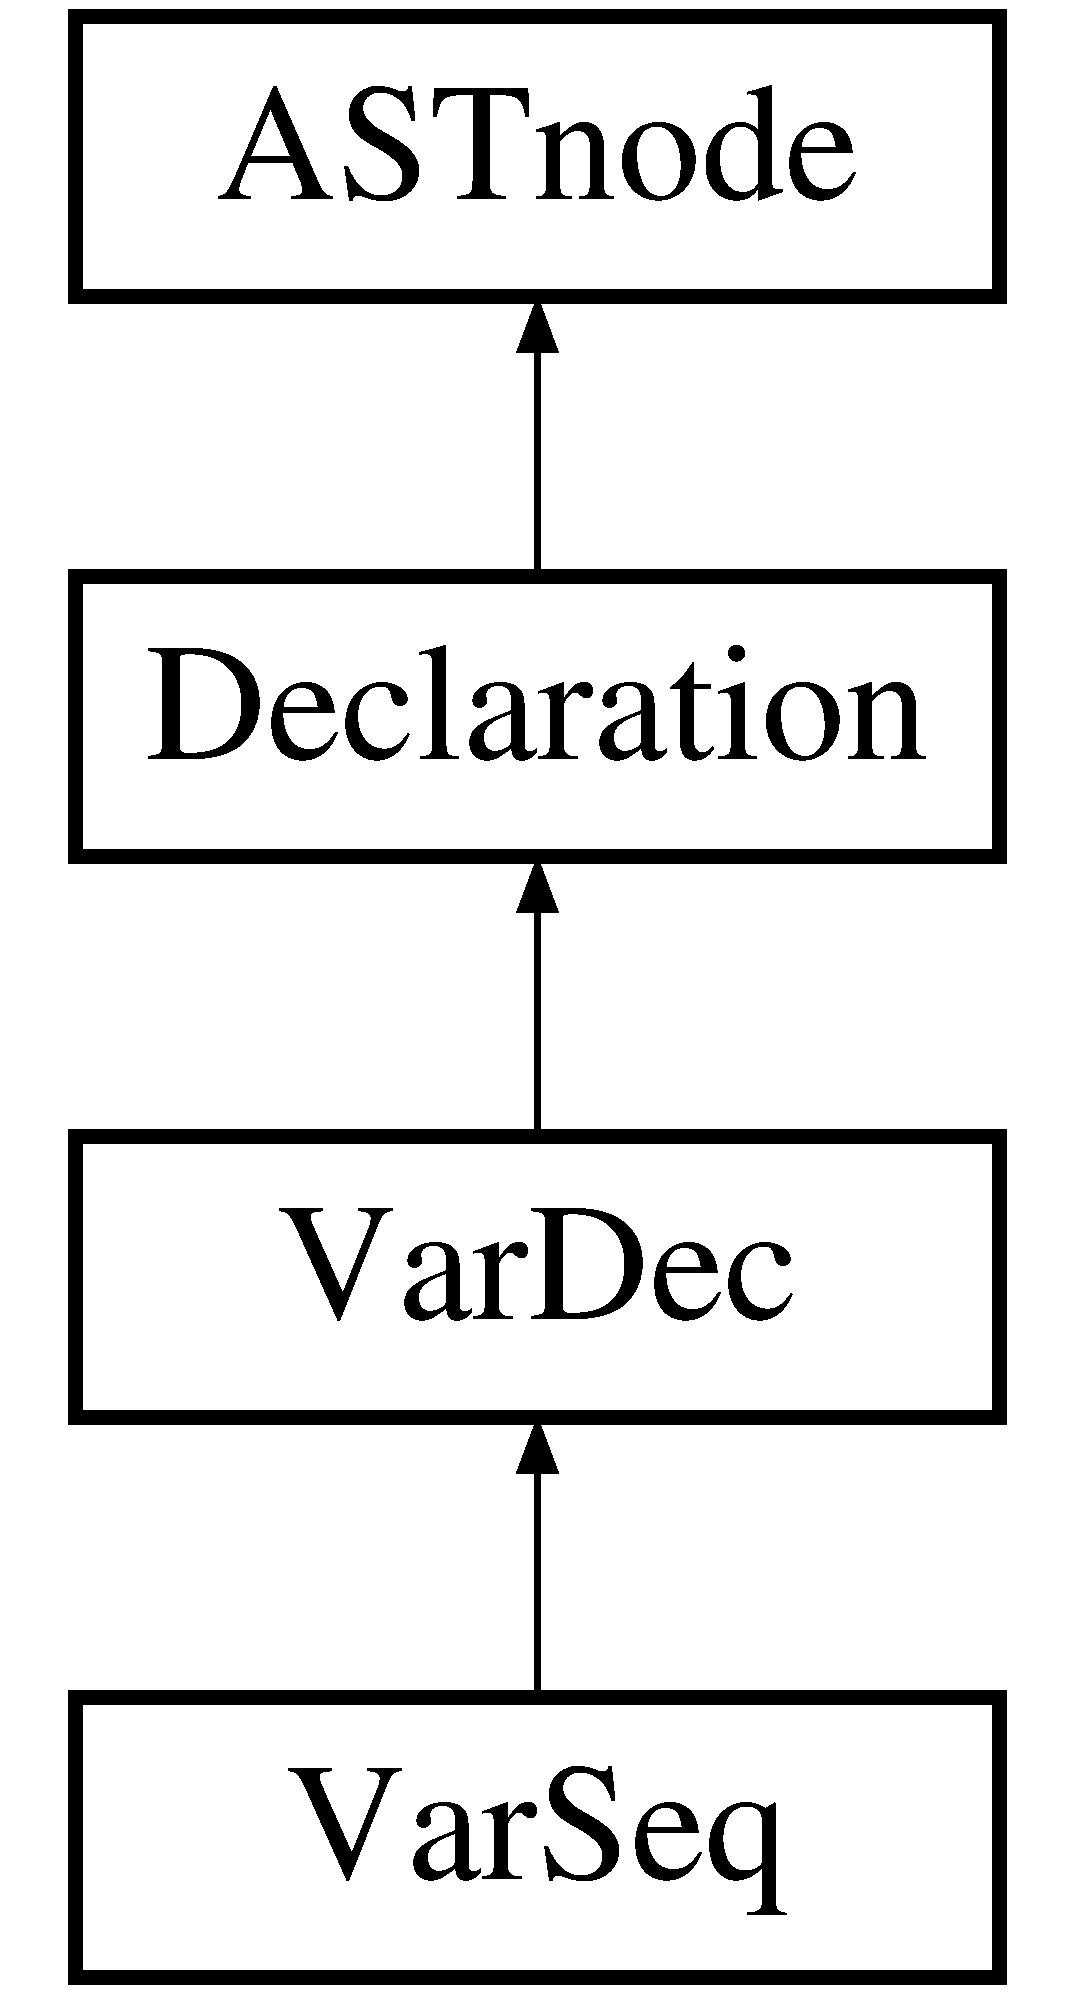
\includegraphics[height=4.000000cm]{class_var_seq}
\end{center}
\end{figure}
\subsection*{Public Member Functions}
\begin{DoxyCompactItemize}
\item 
\mbox{\Hypertarget{class_var_seq_a9b59c03ffa6b921bec75407d6d1818e6}\label{class_var_seq_a9b59c03ffa6b921bec75407d6d1818e6}} 
int {\bfseries get\+Count} () const
\item 
\mbox{\Hypertarget{class_var_seq_a291c63b445d855620158e79adca53ef6}\label{class_var_seq_a291c63b445d855620158e79adca53ef6}} 
const \hyperlink{class_var_dec}{Var\+Dec} $\ast$ {\bfseries get\+Declaration} (unsigned int i) const
\item 
\mbox{\Hypertarget{class_var_seq_af981463560dcf565702c7e514cbabe7f}\label{class_var_seq_af981463560dcf565702c7e514cbabe7f}} 
void {\bfseries add\+Declaration} (\hyperlink{class_var_dec}{Var\+Dec} $\ast$state)
\item 
\mbox{\Hypertarget{class_var_seq_acf8a0949a412299c55a91941d3003319}\label{class_var_seq_acf8a0949a412299c55a91941d3003319}} 
void {\bfseries print} () const override
\item 
\mbox{\Hypertarget{class_var_seq_aef8e8eb8d90e1729169b05620508d52a}\label{class_var_seq_aef8e8eb8d90e1729169b05620508d52a}} 
void {\bfseries compile} (\hyperlink{class_context}{Context} \&ctxt, unsigned int dest\+Loc) const override
\end{DoxyCompactItemize}
\subsection*{Additional Inherited Members}


The documentation for this class was generated from the following files\+:\begin{DoxyCompactItemize}
\item 
ast.\+hpp\item 
ast.\+cpp\end{DoxyCompactItemize}

\hypertarget{class_while_statement}{}\section{While\+Statement Class Reference}
\label{class_while_statement}\index{While\+Statement@{While\+Statement}}
Inheritance diagram for While\+Statement\+:\begin{figure}[H]
\begin{center}
\leavevmode
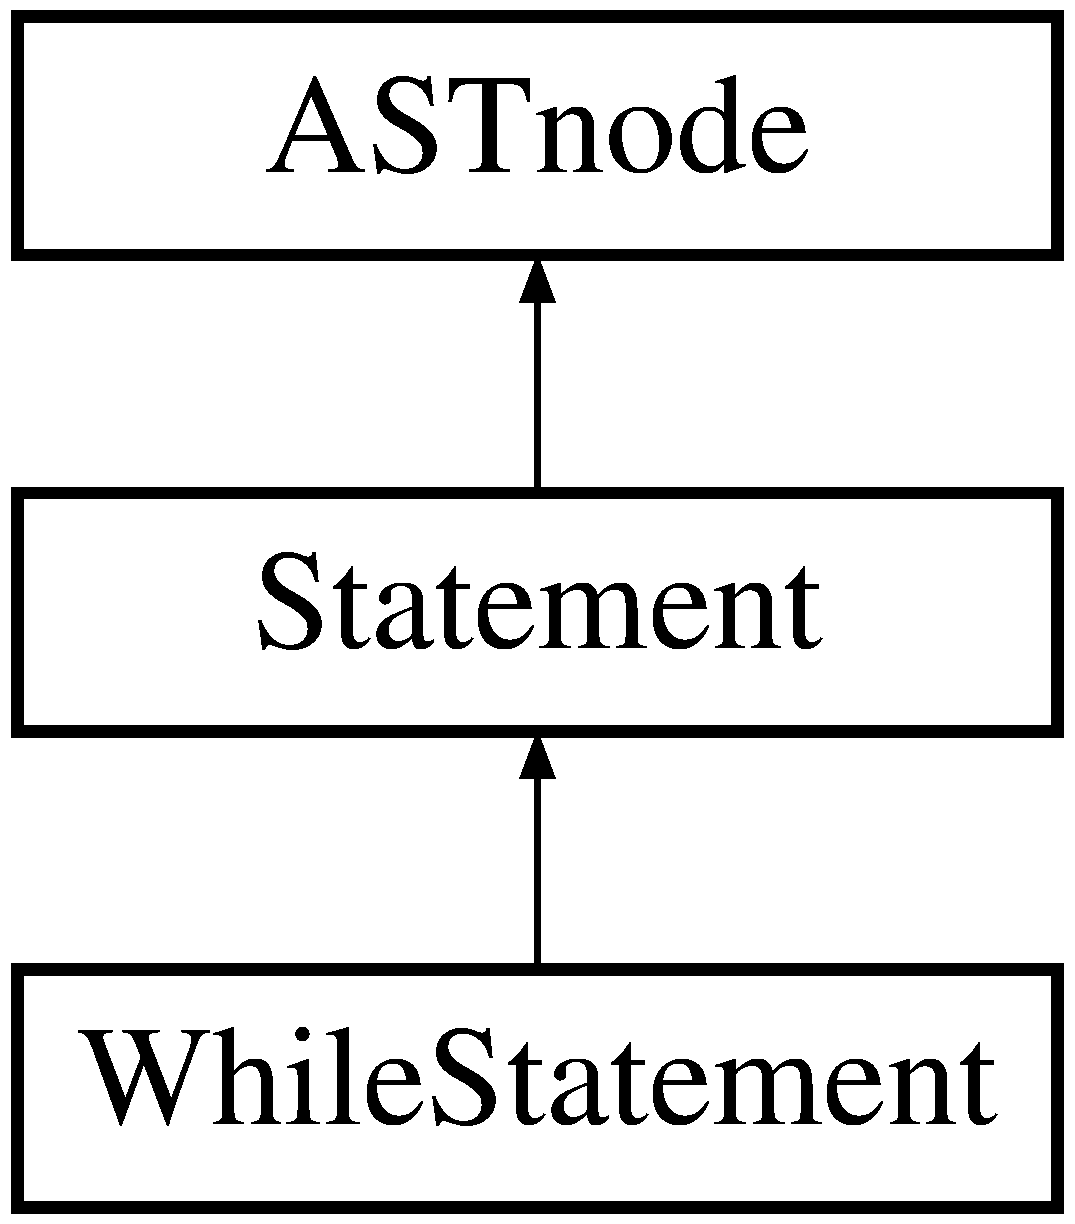
\includegraphics[height=3.000000cm]{class_while_statement}
\end{center}
\end{figure}
\subsection*{Public Member Functions}
\begin{DoxyCompactItemize}
\item 
\mbox{\Hypertarget{class_while_statement_a7900c38944115fd7ba2452d0f2e73b1c}\label{class_while_statement_a7900c38944115fd7ba2452d0f2e73b1c}} 
{\bfseries While\+Statement} (const \hyperlink{class_expression}{Expression} $\ast$cond\+\_\+in, \hyperlink{class_scope}{Scope} $\ast$body\+\_\+in)
\item 
\mbox{\Hypertarget{class_while_statement_afa5b82ee367e5bf02961c057649956e1}\label{class_while_statement_afa5b82ee367e5bf02961c057649956e1}} 
void {\bfseries print} () const override
\item 
\mbox{\Hypertarget{class_while_statement_ab4c3557af0eec74c6c3ae69b98435a9a}\label{class_while_statement_ab4c3557af0eec74c6c3ae69b98435a9a}} 
void {\bfseries compile} (\hyperlink{class_context}{Context} \&ctxt, unsigned int dest\+Loc) const override
\end{DoxyCompactItemize}
\subsection*{Public Attributes}
\begin{DoxyCompactItemize}
\item 
\mbox{\Hypertarget{class_while_statement_a5ae7976e8c7cf064385a05abc441c94e}\label{class_while_statement_a5ae7976e8c7cf064385a05abc441c94e}} 
const \hyperlink{class_expression}{Expression} $\ast$ {\bfseries condition}
\item 
\mbox{\Hypertarget{class_while_statement_a3abdc30265556f0a7e801a0c5fdcee03}\label{class_while_statement_a3abdc30265556f0a7e801a0c5fdcee03}} 
\hyperlink{class_scope}{Scope} $\ast$ {\bfseries body}
\end{DoxyCompactItemize}


The documentation for this class was generated from the following files\+:\begin{DoxyCompactItemize}
\item 
ast.\+hpp\item 
ast.\+cpp\end{DoxyCompactItemize}

\hypertarget{structyy__buffer__state}{}\section{yy\+\_\+buffer\+\_\+state Struct Reference}
\label{structyy__buffer__state}\index{yy\+\_\+buffer\+\_\+state@{yy\+\_\+buffer\+\_\+state}}
\subsection*{Public Attributes}
\begin{DoxyCompactItemize}
\item 
\mbox{\Hypertarget{structyy__buffer__state_a4843d1422e3276b636d475a3095bd948}\label{structyy__buffer__state_a4843d1422e3276b636d475a3095bd948}} 
F\+I\+LE $\ast$ {\bfseries yy\+\_\+input\+\_\+file}
\item 
\mbox{\Hypertarget{structyy__buffer__state_ad7b8df8d8a4688e57b0b8d3ca75adc85}\label{structyy__buffer__state_ad7b8df8d8a4688e57b0b8d3ca75adc85}} 
char $\ast$ {\bfseries yy\+\_\+ch\+\_\+buf}
\item 
\mbox{\Hypertarget{structyy__buffer__state_a58aa927f098b99d99e75da80f9b681ef}\label{structyy__buffer__state_a58aa927f098b99d99e75da80f9b681ef}} 
char $\ast$ {\bfseries yy\+\_\+buf\+\_\+pos}
\item 
\mbox{\Hypertarget{structyy__buffer__state_a48302f5f3477a9c78bbddf56d356ef54}\label{structyy__buffer__state_a48302f5f3477a9c78bbddf56d356ef54}} 
yy\+\_\+size\+\_\+t {\bfseries yy\+\_\+buf\+\_\+size}
\item 
\mbox{\Hypertarget{structyy__buffer__state_a06406208824817acfec2183b79080945}\label{structyy__buffer__state_a06406208824817acfec2183b79080945}} 
int {\bfseries yy\+\_\+n\+\_\+chars}
\item 
\mbox{\Hypertarget{structyy__buffer__state_a80ce2431c70dc4f89ced487f18449465}\label{structyy__buffer__state_a80ce2431c70dc4f89ced487f18449465}} 
int {\bfseries yy\+\_\+is\+\_\+our\+\_\+buffer}
\item 
\mbox{\Hypertarget{structyy__buffer__state_abf5c70eea75581b58c0ee7bd31b14490}\label{structyy__buffer__state_abf5c70eea75581b58c0ee7bd31b14490}} 
int {\bfseries yy\+\_\+is\+\_\+interactive}
\item 
\mbox{\Hypertarget{structyy__buffer__state_a9d60c60af6e1a6f69de16871fd64f85f}\label{structyy__buffer__state_a9d60c60af6e1a6f69de16871fd64f85f}} 
int {\bfseries yy\+\_\+at\+\_\+bol}
\item 
int \hyperlink{structyy__buffer__state_a818e94bc9c766e683c60df1e9fd01199}{yy\+\_\+bs\+\_\+lineno}
\item 
int \hyperlink{structyy__buffer__state_a10c4fcd8be759e6bf11e6d3e8cdb0307}{yy\+\_\+bs\+\_\+column}
\item 
\mbox{\Hypertarget{structyy__buffer__state_a63d2afbb1d79a3fc63df9e12626f827d}\label{structyy__buffer__state_a63d2afbb1d79a3fc63df9e12626f827d}} 
int {\bfseries yy\+\_\+fill\+\_\+buffer}
\item 
\mbox{\Hypertarget{structyy__buffer__state_a70fd925d37a2f0454fbd0def675d106c}\label{structyy__buffer__state_a70fd925d37a2f0454fbd0def675d106c}} 
int {\bfseries yy\+\_\+buffer\+\_\+status}
\end{DoxyCompactItemize}


\subsection{Member Data Documentation}
\mbox{\Hypertarget{structyy__buffer__state_a10c4fcd8be759e6bf11e6d3e8cdb0307}\label{structyy__buffer__state_a10c4fcd8be759e6bf11e6d3e8cdb0307}} 
\index{yy\+\_\+buffer\+\_\+state@{yy\+\_\+buffer\+\_\+state}!yy\+\_\+bs\+\_\+column@{yy\+\_\+bs\+\_\+column}}
\index{yy\+\_\+bs\+\_\+column@{yy\+\_\+bs\+\_\+column}!yy\+\_\+buffer\+\_\+state@{yy\+\_\+buffer\+\_\+state}}
\subsubsection{\texorpdfstring{yy\+\_\+bs\+\_\+column}{yy\_bs\_column}}
{\footnotesize\ttfamily int yy\+\_\+buffer\+\_\+state\+::yy\+\_\+bs\+\_\+column}

The column count. \mbox{\Hypertarget{structyy__buffer__state_a818e94bc9c766e683c60df1e9fd01199}\label{structyy__buffer__state_a818e94bc9c766e683c60df1e9fd01199}} 
\index{yy\+\_\+buffer\+\_\+state@{yy\+\_\+buffer\+\_\+state}!yy\+\_\+bs\+\_\+lineno@{yy\+\_\+bs\+\_\+lineno}}
\index{yy\+\_\+bs\+\_\+lineno@{yy\+\_\+bs\+\_\+lineno}!yy\+\_\+buffer\+\_\+state@{yy\+\_\+buffer\+\_\+state}}
\subsubsection{\texorpdfstring{yy\+\_\+bs\+\_\+lineno}{yy\_bs\_lineno}}
{\footnotesize\ttfamily int yy\+\_\+buffer\+\_\+state\+::yy\+\_\+bs\+\_\+lineno}

The line count. 

The documentation for this struct was generated from the following file\+:\begin{DoxyCompactItemize}
\item 
lexer.\+yy.\+cpp\end{DoxyCompactItemize}

\hypertarget{structyy__trans__info}{}\section{yy\+\_\+trans\+\_\+info Struct Reference}
\label{structyy__trans__info}\index{yy\+\_\+trans\+\_\+info@{yy\+\_\+trans\+\_\+info}}
\subsection*{Public Attributes}
\begin{DoxyCompactItemize}
\item 
\mbox{\Hypertarget{structyy__trans__info_a5c9f61e770deef50bd4e697310342fe9}\label{structyy__trans__info_a5c9f61e770deef50bd4e697310342fe9}} 
flex\+\_\+int32\+\_\+t {\bfseries yy\+\_\+verify}
\item 
\mbox{\Hypertarget{structyy__trans__info_ae0715250c2bef261e596e77e0030f13e}\label{structyy__trans__info_ae0715250c2bef261e596e77e0030f13e}} 
flex\+\_\+int32\+\_\+t {\bfseries yy\+\_\+nxt}
\end{DoxyCompactItemize}


The documentation for this struct was generated from the following file\+:\begin{DoxyCompactItemize}
\item 
lexer.\+yy.\+cpp\end{DoxyCompactItemize}

\hypertarget{unionyyalloc}{}\section{yyalloc Union Reference}
\label{unionyyalloc}\index{yyalloc@{yyalloc}}
\subsection*{Public Attributes}
\begin{DoxyCompactItemize}
\item 
\mbox{\Hypertarget{unionyyalloc_a4800e0520a89a4789afa7b5d82197e65}\label{unionyyalloc_a4800e0520a89a4789afa7b5d82197e65}} 
yytype\+\_\+int16 {\bfseries yyss\+\_\+alloc}
\item 
\mbox{\Hypertarget{unionyyalloc_a9326f4fdc6f737a929444427836d8928}\label{unionyyalloc_a9326f4fdc6f737a929444427836d8928}} 
\hyperlink{union_y_y_s_t_y_p_e}{Y\+Y\+S\+T\+Y\+PE} {\bfseries yyvs\+\_\+alloc}
\end{DoxyCompactItemize}


The documentation for this union was generated from the following file\+:\begin{DoxyCompactItemize}
\item 
parser.\+tab.\+cpp\end{DoxyCompactItemize}

\hypertarget{union_y_y_s_t_y_p_e}{}\section{Y\+Y\+S\+T\+Y\+PE Union Reference}
\label{union_y_y_s_t_y_p_e}\index{Y\+Y\+S\+T\+Y\+PE@{Y\+Y\+S\+T\+Y\+PE}}
\subsection*{Public Attributes}
\begin{DoxyCompactItemize}
\item 
\mbox{\Hypertarget{union_y_y_s_t_y_p_e_a778d76bb998ec04647b59dc4f84e4a56}\label{union_y_y_s_t_y_p_e_a778d76bb998ec04647b59dc4f84e4a56}} 
const \hyperlink{class_a_s_tnode}{A\+S\+Tnode} $\ast$ {\bfseries ast}
\item 
\mbox{\Hypertarget{union_y_y_s_t_y_p_e_ad7df710a3b0ec2941de5517ebb79eefc}\label{union_y_y_s_t_y_p_e_ad7df710a3b0ec2941de5517ebb79eefc}} 
\hyperlink{class_scope}{Scope} $\ast$ {\bfseries scope}
\item 
\mbox{\Hypertarget{union_y_y_s_t_y_p_e_acc8ac22a66d86927f507d0894136865a}\label{union_y_y_s_t_y_p_e_acc8ac22a66d86927f507d0894136865a}} 
\hyperlink{class_param_dec}{Param\+Dec} $\ast$ {\bfseries par\+\_\+dec}
\item 
\mbox{\Hypertarget{union_y_y_s_t_y_p_e_a9e2ec228e56d6bf901820fdf9bc63c89}\label{union_y_y_s_t_y_p_e_a9e2ec228e56d6bf901820fdf9bc63c89}} 
\hyperlink{class_param_seq}{Param\+Seq} $\ast$ {\bfseries par\+\_\+seq}
\item 
\mbox{\Hypertarget{union_y_y_s_t_y_p_e_ad95e9a1c0e72429a6790de8a9c12508b}\label{union_y_y_s_t_y_p_e_ad95e9a1c0e72429a6790de8a9c12508b}} 
\hyperlink{class_arg_seq}{Arg\+Seq} $\ast$ {\bfseries arg\+\_\+seq}
\item 
\mbox{\Hypertarget{union_y_y_s_t_y_p_e_a71aa26f8f6bd1b239d40b8fa089492a2}\label{union_y_y_s_t_y_p_e_a71aa26f8f6bd1b239d40b8fa089492a2}} 
\hyperlink{class_var_dec}{Var\+Dec} $\ast$ {\bfseries var\+\_\+dec}
\item 
\mbox{\Hypertarget{union_y_y_s_t_y_p_e_a71753ca94bd18ddd2de885fe0688b190}\label{union_y_y_s_t_y_p_e_a71753ca94bd18ddd2de885fe0688b190}} 
\hyperlink{class_var_seq}{Var\+Seq} $\ast$ {\bfseries var\+\_\+seq}
\item 
\mbox{\Hypertarget{union_y_y_s_t_y_p_e_a4bea199471379902fe0a89cfdff31b1e}\label{union_y_y_s_t_y_p_e_a4bea199471379902fe0a89cfdff31b1e}} 
const \hyperlink{class_expression}{Expression} $\ast$ {\bfseries expression}
\item 
\mbox{\Hypertarget{union_y_y_s_t_y_p_e_a3a91e31e5e63f3d04553e8c84a03a439}\label{union_y_y_s_t_y_p_e_a3a91e31e5e63f3d04553e8c84a03a439}} 
\hyperlink{class_statement}{Statement} $\ast$ {\bfseries statement}
\item 
\mbox{\Hypertarget{union_y_y_s_t_y_p_e_aa0e6b4c9b798fc61cc9e62c5b74f68f6}\label{union_y_y_s_t_y_p_e_aa0e6b4c9b798fc61cc9e62c5b74f68f6}} 
\hyperlink{class_statement_sequence}{Statement\+Sequence} $\ast$ {\bfseries statement\+\_\+sequence}
\item 
\mbox{\Hypertarget{union_y_y_s_t_y_p_e_a2c6e041cfb542764b8c40a8f3bb9cf51}\label{union_y_y_s_t_y_p_e_a2c6e041cfb542764b8c40a8f3bb9cf51}} 
const std\+::string $\ast$ {\bfseries my\+\_\+string}
\item 
\mbox{\Hypertarget{union_y_y_s_t_y_p_e_a5d46ca0a0ad5ea95c057b764a95fdd21}\label{union_y_y_s_t_y_p_e_a5d46ca0a0ad5ea95c057b764a95fdd21}} 
const int $\ast$ {\bfseries my\+\_\+int}
\end{DoxyCompactItemize}


The documentation for this union was generated from the following files\+:\begin{DoxyCompactItemize}
\item 
parser.\+tab.\+cpp\item 
parser.\+tab.\+hpp\end{DoxyCompactItemize}

%--- End generated contents ---

% Index
\backmatter
\newpage
\phantomsection
\clearemptydoublepage
\addcontentsline{toc}{chapter}{Index}
\printindex

\end{document}
